\documentclass[11pt]{report}

\usepackage[T1]{fontenc}
\usepackage[utf8]{inputenc}
\usepackage{lmodern}
\usepackage{amsmath,amssymb,mathtools}
\usepackage{microtype}
\usepackage{hyperref}
\usepackage{geometry}
\geometry{margin=1in, footskip=0.5in}
\usepackage{setspace}        % USC requires double spacing
\doublespacing
\usepackage{upquote}
\usepackage{graphicx}
\usepackage{wrapfig}
\usepackage{float}
\graphicspath{{Dissertation_images/}}
\usepackage[font=small,singlelinecheck=false]{caption}
\usepackage{enumitem}         % For glossary formatting

\DeclareMathOperator{\diag}{\mathrm{diag}}
\DeclareMathOperator{\tr}{tr}
\newcommand{\R}{\mathbb{R}}
\newcommand{\M}{\mathbb{M}}

\begin{document}

% ===== TITLE PAGE (no page number) =====
% USC PhD template — do not bold text or add extraneous information
\thispagestyle{empty}
\begin{center}
\vspace*{1in}

Next-Generation Hyperspectral Remote Sensing Data Processing:\\
Efficient and Scalable Workflows Integrating Transformer Architectures,\\
Physics-Informed Priors, and Statistical Learning

\vspace{0.5in}
by

\vspace{0.5in}
Kelli McCoy

\vspace{1in}
A Dissertation Presented to the\\
FACULTY OF THE USC GRADUATE SCHOOL\\
UNIVERSITY OF SOUTHERN CALIFORNIA\\
In Partial Fulfillment of the\\
Requirements for the Degree\\
DOCTOR OF PHILOSOPHY\\
(ENVIRONMENTAL ENGINEERING)

\vspace{0.75in}
August 2026

\end{center}

\vfill
\noindent Copyright 2026 \hfill Kelli McCoy

\newpage

% ===== PRELIMINARY PAGES (lowercase Roman numerals, starting at ii) =====
\pagenumbering{roman}
\setcounter{page}{2}

% --- Dedication ---
\chapter*{Dedication}
\addcontentsline{toc}{chapter}{Dedication}

\vspace*{2in}
\begin{center}
\textit{To my husband, James, for his tireless support and sacrifice over the past five years.}
\end{center}

\newpage

% --- Acknowledgements ---
\chapter*{Acknowledgements}
\addcontentsline{toc}{chapter}{Acknowledgements}

% TODO: Add your acknowledgements here
I would like to thank my Advisor, Professor Roger Ghanem, for his guidance and support throughout this research. 



\newpage

% --- Table of Contents ---
\tableofcontents
\newpage

% --- List of Tables ---
\listoftables
\addcontentsline{toc}{chapter}{List of Tables}
\newpage

% --- List of Figures ---
\listoffigures
\addcontentsline{toc}{chapter}{List of Figures}
\newpage

% --- Abstract ---
\chapter*{Abstract}
\addcontentsline{toc}{chapter}{Abstract}

The increasing volume of hyperspectral data from missions like NASA's EMIT necessitates a shift toward computationally efficient, scalable processing. Traditional radiative transfer model (RTM)-based atmospheric correction faces high latency and generalization challenges, limiting the pace of science delivery and the ability to make timely operational decisions such as targeted revisits. This dissertation proposes an integrated framework that classifies minerals directly from L1B radiance or top-of-atmosphere (TOA) reflectance, bypassing RTM-based atmospheric correction entirely, by fusing Transformer architectures with physics-based and statistical learning methods to optimize mineral identification.

Central to this workflow is a Transformer-based multi-head attention pooling model that captures complex spectral dependencies across all 285 EMIT bands simultaneously, reducing computational complexity from $O(L^2)$ to $O(H \times L)$. To address spectroscopic interpretability, the architecture incorporates PCA-derived spectral priors from USGS reference mineral spectra to initialize attention heads toward known diagnostic absorption features. Per-head attention analysis reveals that the model independently discovers spectroscopically valid features, validated by peak coincidence within $\pm$20~nm of literature values, providing interpretable evidence that the learned representations are physically meaningful. Learning Using Statistical Invariants (LUSI), inspired by Vapnik's complete statistical learning theory, enforces illumination and atmospheric invariance through consistency regularization, maintaining or improving classification performance on geographically independent test scenes, consistent with the theory that statistical invariants provide the greatest benefit when test conditions differ from training. The attention-derived band importance rankings support intelligent data prioritization --- identifying which spectral bands carry the most discriminative information enables targeted data volume reduction without sacrificing classification reliability.

To address the scenario of limited training data, the framework implements Probabilistic Learning on Manifolds (PLoM), which discovers the diffusion manifold underlying a small initial dataset of SDS-processed spectral samples and generates additional statistically representative realizations, constrained to fluctuate in the neighborhood of this manifold. This manifold-based augmentation preserves the joint probability distribution of spectral signatures, enabling the training of high-capacity models from minimal labeled data. To further address the curse of dimensionality, the framework implements Knockoff feature selection, providing a statistically rigorous method to identify truly informative spectral bands while controlling the false discovery rate. Methods are applied at both the full image level, classifying entire EMIT scenes in a single inference pass, as well as the pixel-by-pixel conventional approach.

Experimental results demonstrate that this fusion of attention-based learning, physics-informed spectral priors, statistical invariance regularization, knockoff-driven band selection, and manifold-based data generation reduces computational overhead while maintaining high mineral classification reliability across desert regions of the globe. The sensor-agnostic architecture is extensible beyond EMIT to other hyperspectral platforms. By eliminating the RTM bottleneck and enabling rapid scene-level inference, this framework reduces science turnaround time and mission operations cost, and establishes a foundation for onboard or edge-based processing where low-latency mineral classification could support autonomous revisit decisions and real-time science prioritization. This research provides a scalable pathway for efficient global mineral mapping and hyperspectral retrieval, overcoming the traditional trade-off between physical rigor and processing speed.

\newpage

% ===== MAIN BODY (Arabic numerals, starting at 1) =====
\pagenumbering{arabic}

% ######################################################################
% CHAPTER 1: INTRODUCTION
% ######################################################################
\chapter{Introduction and Problem Framing}
\label{chap:intro}

This chapter establishes the context, motivation, and objectives for the research presented in this dissertation.
It begins by introducing the critical role of hyperspectral remote sensing, focusing in on climate modeling.
NASA's Earth Surface Mineral Dust Source Investigation (EMIT) mission is highlighted as its cornerstone mineralogy mission, quantifying mineral dust radiative forcing to improve global climate models.
Subsequently, it identifies the computational bottlenecks and limitations inherent in current physics-based data processing pipelines when tasked with handling petabyte-scale, high-dimensional data cubes.
To address these challenges, this chapter formalizes the problem statement, introduces the RTM-bypass paradigm that unifies both parts of this dissertation, and outlines the core research objectives.

\section{Motivation and Context}

Satellites are informing climate conclusions with measurements taken hundreds of kilometers above the Earth’s surface, through Earth’s atmosphere, without direct contact with their subject of interest. 
This is achieved through sensors, mounted on satellites, aircraft, or other platforms, which collect data across various spectral bands by measuring electromagnetic radiation that is emitted, reflected, or scattered by the surface target. 
Data is then analyzed to extract meaningful information about the subject (on Earth's surface).
The data collected by these systems enable us to observe processes over time and space scales that are otherwise unattainable, providing critical insights into phenomena such as deforestation, atmospheric pollution, and ocean health.

Figure~\ref{fig:fleet} depicts many of NASA’s operational space missions observing Earth today.
NASA’s Earth Observing System Data and Information System (EOSDIS) archives and distributes data from various Earth-observing missions. 
As of fiscal year 2025, the total archive volume exceeded 178.7 PB, with an average daily growth of approximately 160 TB \cite{nasa_earthdata_2025}.

% Changed [htbp] to [H] to force exact placement
\begin{figure}[htbp]
\centering
    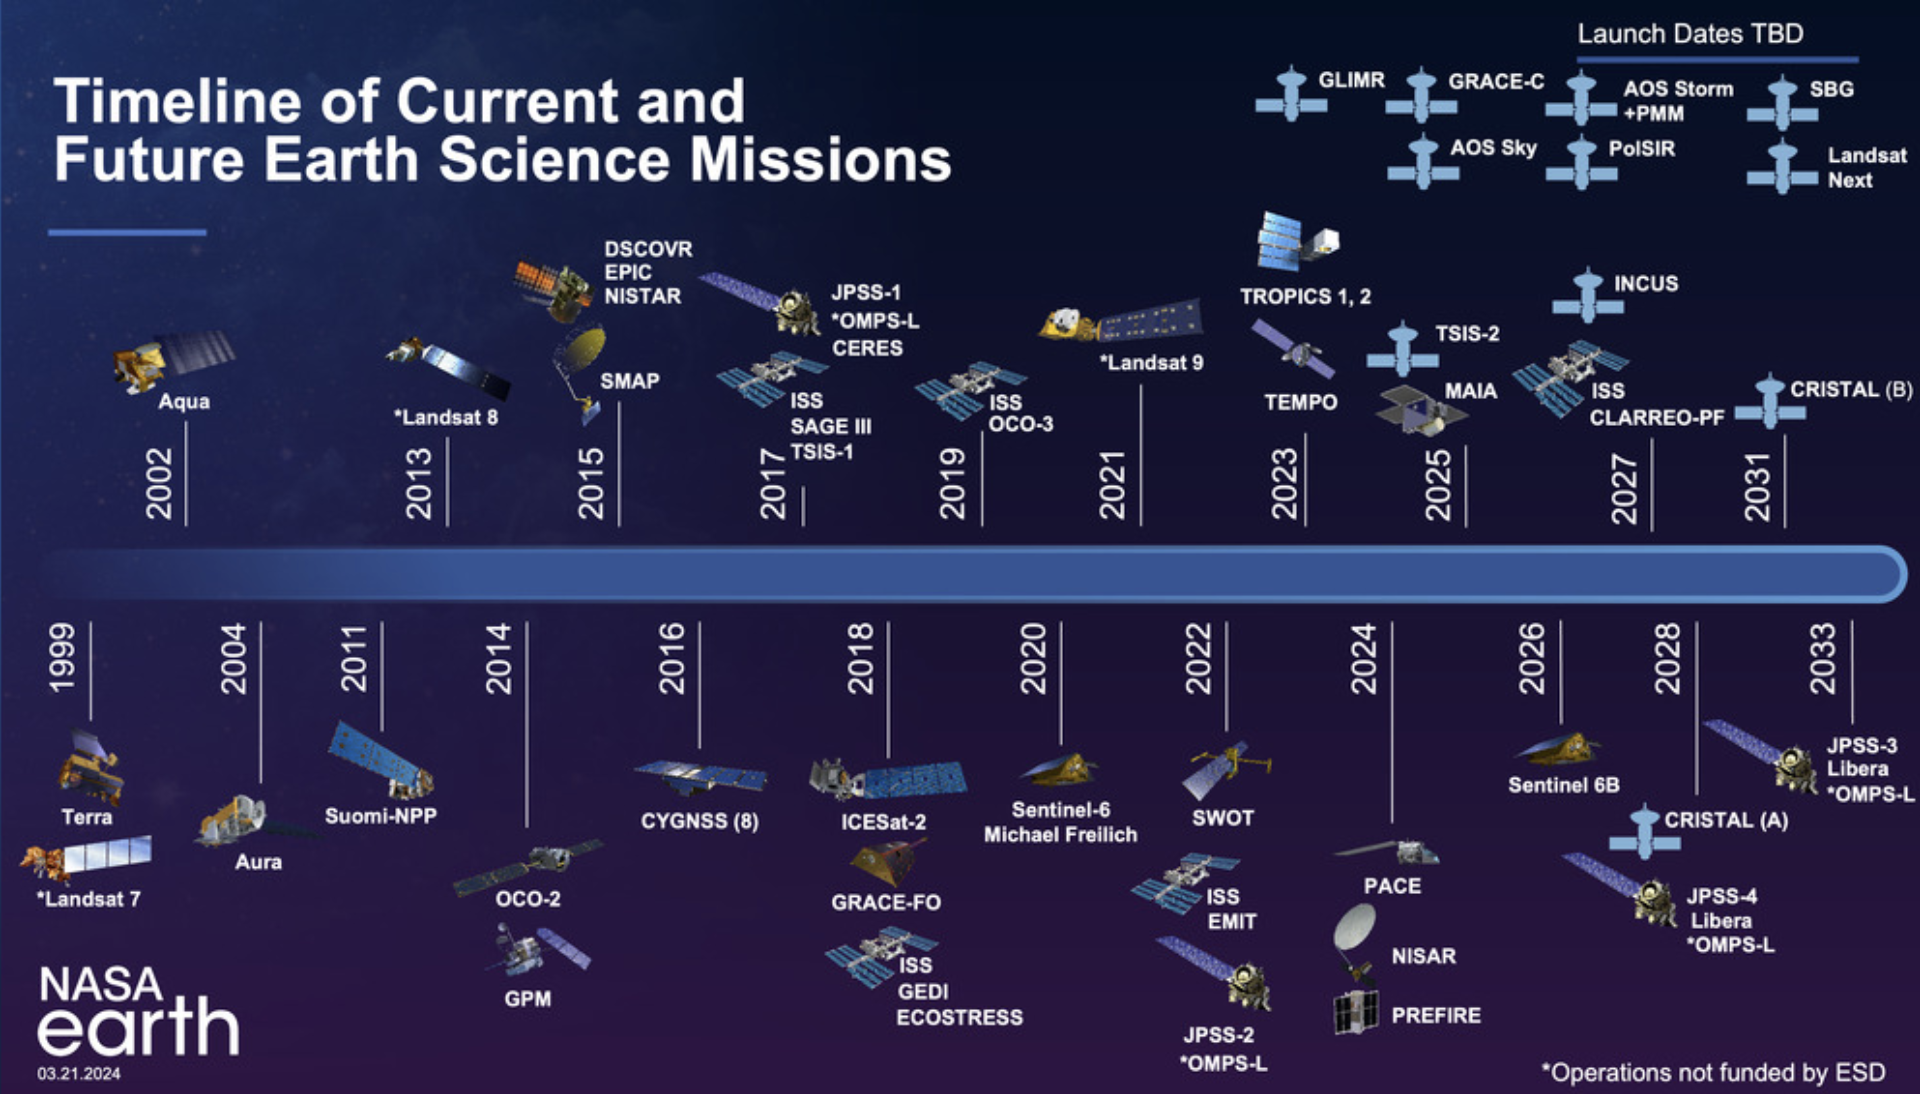
\includegraphics[width=\textwidth]{CurrentandFutureEarthScienceMissions_asof11132025.png}
    % This pulls the caption up closer to the image
    \vspace{-20pt} 
    \caption{\small NASA's Earth Science fleet as of 2025. Image courtesy of NASA Scientific Visualization Studio \cite{nasa_svs_fleet}.}
    \label{fig:fleet}
    % This pulls the following text up closer to the caption
    \vspace{-10pt}
\end{figure}

The rapidly growing number of Earth observing missions has resulted in an unprecedented surge in the volume and complexity of remote sensing data. 
Modern sensors produce high-dimensional datasets, including hyperspectral imagery and multi-angle observations, which require advanced processing methods. 
Despite these advancements, existing pipelines face significant challenges in efficiently handling these data streams while ensuring the quality and reliability of the derived products.

Imaging spectrometers, often referred to as hyperspectral sensors, acquire rasters of spectra to map geophysical phenomena \cite{thompson_emit_2024}. 
Unlike traditional multispectral instruments that measure light in a few broad, discrete bands, imaging spectrometers capture electromagnetic radiation across hundreds of narrow, contiguous spectral channels. 
This continuous sampling produces a three-dimensional ``data cube'' consisting of two spatial dimensions ($x, y$) and one high-dimensional spectral dimension ($\lambda$). 
Consequently, every spatial pixel contains a detailed spectral signature, a unique optical fingerprint, that allows for the identification and quantification of surface materials. 
Identifying these materials heavily relies on comparing orbital measurements against comprehensive reference databases, notably the United States Geological Survey (USGS) Spectral Library \cite{kokaly2017usgs}. 
This library provides the foundational, laboratory-measured pure spectral signatures required to classify and map minerals globally.
Because of this rich information content and established reference data, these instruments have been utilized to study terrestrial and aquatic ecosystems, mineral and water resources, greenhouse gas point sources, and more.
While the first imaging spectrometers were developed over 40 years ago \cite{goetz1985}, the technology has recently reached a new stage of maturity, culminating in advanced orbital instruments capable of conducting continuous, high-fidelity global investigations \cite{thompson_emit_2024}.

While instruments like EMIT are revolutionizing our understanding of surface mineralogy and dust-climate interactions, the high-dimensional data cubes produced by hyperspectral imaging are unlocking capabilities across a wide array of domains. 
The ability to capture continuous, narrow bands across the electromagnetic spectrum allows for precise material identification that standard multispectral sensors cannot match. 
Several major application areas illustrate this breadth:

\paragraph{Precision agriculture and forestry.}
HSI is utilized to monitor plant health at a chemical level, often detecting stress before it becomes visible to the human eye. 
Specific spectral signatures associated with water stress, nutrient deficiencies (nitrogen, phosphorus), or early-stage fungal infections can be identified from airborne or satellite platforms. 
In forestry, HSI enables mapping of complex ecosystems by distinguishing between subtle variations in tree species and tracking the spread of invasive plants. 
Crop biochemical traits can be analyzed to optimize harvesting schedules and predict agricultural yield.

\paragraph{Medical diagnostics and biomedical imaging.}
The medical field is increasingly adopting HSI for non-invasive, real-time tissue analysis. 
In surgical guidance, HSI helps define tumor margins by distinguishing between the spectral signatures of healthy and cancerous tissue. 
Tissue viability assessment, measuring oxygen saturation and blood perfusion, is critical for burn triage, diabetic foot ulcer management, and transplant monitoring. 
Retinal imaging applications detect early signs of degenerative eye diseases by mapping the biochemical composition of the retina.

\paragraph{Planetary science and space exploration.}
HSI is a primary tool for understanding the composition of other celestial bodies. 
Orbiters use hyperspectral instruments to map the mineralogy of the Moon, Mars, and asteroids, identifying resources such as water-ice or rare earth elements that could support future in-situ resource utilization (ISRU). 
For ocean worlds like Europa and Enceladus, HSI enables identification of surface salts and organics to assess habitability.

\paragraph{Defense, intelligence, and security.}
The ability to differentiate between visually identical materials makes HSI valuable for security applications. 
Camouflage detection exploits the fact that artificial materials and natural backgrounds, though identical in the visible spectrum,have drastically different hyperspectral signatures. 
Chemical and biological threat detection leverages the specific absorption features of hazardous gases or chemical spills to enable identification from standoff distances.

\paragraph{Industrial sorting and food quality.}
High-speed HSI cameras are integrated into automated machine-vision pipelines for quality control. 
In food safety, HSI detects sub-surface bruising on fruit, identifies aflatoxin contamination in grains, and locates foreign materials in processing lines. 
Waste recycling applications use near-infrared spectral properties to rapidly sort optically similar plastics (e.g., PET vs.\ PVC), improving recycling efficiency.

Because all of these applications generate massive, complex datasets, they increasingly rely on scalable processing workflows and advanced statistical methods to achieve real-time predictive analytics. 
The computational challenges addressed in this dissertation---efficient dimensionality reduction, physics-informed feature extraction, and RTM-bypass inference---are therefore relevant well beyond the mineral classification problem that motivates the specific methods developed here.

Mineral dust radiative forcing, the measure of how airborne dust alters the Earth's energy balance by scattering or absorbing sunlight, is one of the largest uncertainties in climate modeling \cite{ipcc_2021}. 
This forcing profoundly impacts regional climates, driving changes in agriculture, precipitation, and desert encroachment. 
The net effect of a dust plume depends heavily on its mineral composition. 
Light-colored minerals (e.g., clays and quartz) reflect sunlight and cool the atmosphere, whereas dark-colored minerals (specifically iron oxides like hematite) absorb solar energy and generate heat. 

\setlength{\columnsep}{15pt}
\begin{wrapfigure}{L}{0.5\textwidth} 
    \vspace{-2mm} 
    \centering
    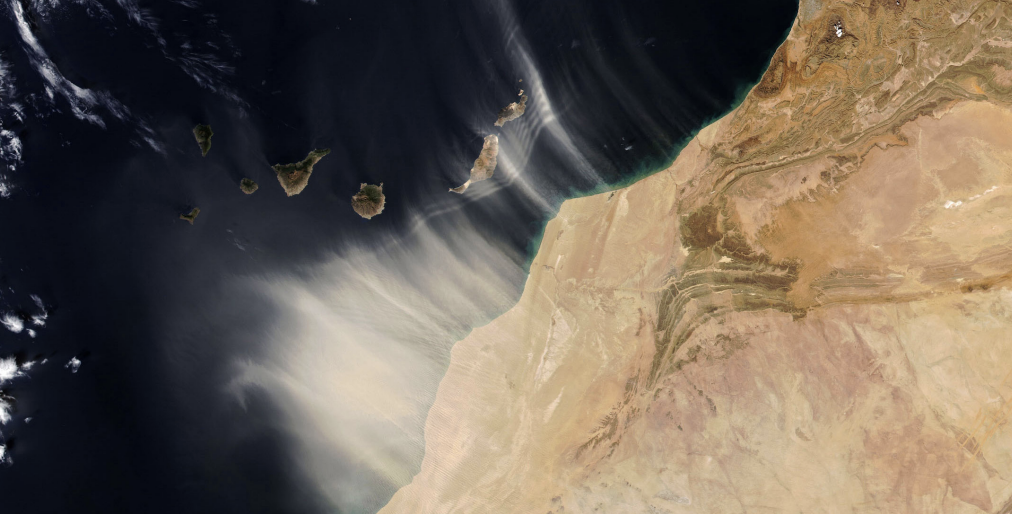
\includegraphics[width=\linewidth]{EMIT_dust.png}
    \vspace{-6mm}
    \caption{\small NASA’s EMIT mission studies the composition of surface minerals in Earth’s arid regions, helping climate researchers better understand how dust affects climate when it is blown into the atmosphere. \cite{emit_factsheet}}
    \label{fig:emit_dust}
    \vspace{-2mm}
\end{wrapfigure}

Because current climate models often rely on highly uncertain estimates of iron oxide abundance (ranging from $0$ to $7\text{ wt}\%$), they can produce up to a $460\%$ uncertainty in regional radiative forcing predictions.
Meanwhile, physical soil samples from critical dust sources like North Africa reveal up to $30\text{ wt}\%$ iron oxide \cite{emit_l1b_atbd}.
To close this critical knowledge gap, NASA competitively selected and developed the Earth Surface Mineral Dust Source Investigation (EMIT).

EMIT maps the mineral composition of Earth's arid regions, providing the precise data needed to understand the true climatic impact of airborne dust.
Mounted aboard the International Space Station (ISS) 400km above Earth, EMIT collects hyperspectral data on the composition and color of surface minerals across Earth’s most dust-productive regions (depicted in Figure~\ref{fig:emit_dust}). 
Using a state-of-the-art imaging spectrometer operating in the visible to shortwave infrared (VSWIR) spectrum, EMIT provides the first global maps detailing the abundance of ten key minerals: hematite, goethite, illite, vermiculite, calcite, dolomite, montmorillonite, kaolinite, chlorite, and gypsum. 
Each of these minerals affects the absorption and reflection of solar radiation differently, influencing the climatic effects of airborne dust.

However, translating these massive, complex hyperspectral data cubes into precise mineralogical maps presents a computational challenge. 
Extracting accurate fractional abundances of these ten key minerals from highly mixed spatial pixels requires moving beyond traditional deterministic spectral matching. 
To fully leverage the unprecedented volume of data provided by missions like EMIT, there is a critical need for efficient, highly scalable workflows capable of learning complex spectral representations, while providing contextual uncertainty.

\section{Limitations of Current Data Pipelines}

The data acquired from remote sensing instruments like EMIT are not direct measurements of surface properties. 
Instead, the observed reflectances are influenced by the interactions of light with gases and particles within the atmosphere, as well as instrument characteristics. 
The process of obtaining meaningful geophysical parameters from remotely sensed data relies heavily on accurate modeling of these interactions through physics-based Radiative Transfer Models (RTMs) and the implementation of robust retrieval algorithms.

These processes face fundamental limitations:
\begin{itemize}
  \item \textbf{Computational Expense:} While they are becoming more physically accurate,  RTMs are correspondingly more computationally demanding, often requiring months of latency, post-delivery, to produce Level~2 geophysical products \cite{emit_l1b_atbd}.
  This latency is incompatible with the rapid science delivery and operational decision-making required for timely revisit scheduling and real-time science prioritization.
  The computational cost of RTM-based retrievals also limits the ability to reprocess data with improved models or to perform large-scale sensitivity analyses.
  For missions like EMIT, which produce sets of petabyte-scale hyperspectral data cubes, the computational burden of RTM-based processing becomes a critical bottleneck that hinders the full scientific exploitation of the data.
  This motivates the development of RTM-emulation or bypass methods that can directly map Level~1 observations to Level~2 products without invoking the full physics-based retrieval process.
  \item \textbf{Heavy reliance on deterministic spectral matching:} Current mineral identification (e.g., Tetracorder \cite{clark2003tetracorder, clark2024tetracorder}) depends on expert-curated rules and reference library matching developed over $\sim$100 person-years. 
  While proven across diverse environments from Earth to Mars, the system requires hand-crafted continuum definitions, feature constraints, and shoulderness thresholds for each reference spectrum, and known issues documents are maintained for each expert system version as new geologic environments reveal deficiencies in the spectral libraries.
  It is difficult to scale this approach to the volume and diversity of data produced by modern hyperspectral missions, and it does not leverage the full information content of the spectra, which may contain subtle features that are not captured by deterministic rules.
  The reliance on deterministic spectral matching also limits the ability to capture complex, non-linear relationships between spectral features and mineralogical composition. 
  The development of data-driven, machine learning-based approaches that can learn complex spectral representations and provide contextual uncertainty is a critical area of research to overcome these limitations and fully exploit the scientific potential of hyperspectral remote sensing data.
  
\end{itemize}
% ## Maybe this moves

The EMIT pipeline illustrates these limitations concretely. 
The most computationally intensive stage is the Level~1B to Level~2A transition, where the ISOFIT software package implements an Optimal Estimation (OE) framework to retrieve surface reflectance by correcting for atmospheric absorption and scattering \cite{thompson2018, emit_l2a_atbd}. 
The retrieval process may not yield a unique solution, and the solution can be highly sensitive to small variations in the input data.
This Bayesian inversion introduces several acknowledged deficiencies:
\begin{itemize}
  \item \textbf{Aerosol Limits:} Observations with aerosol optical depth (AOD) greater than 0.5 at 550~nm are masked and excluded from Level~3 aggregation \cite{emit_l2a_atbd, emit_l3_atbd}. 
  This creates a thematic bottleneck: the very dust source regions EMIT aims to study often experience high aerosol loads that prevent valid reflectance retrieval.
  \item \textbf{Water Vapor Biases:} High-resolution water vapor maps derived from ISOFIT can exhibit spatial standard deviation biases ranging from $-$7\% to $+$34\%, primarily related to assumed atmospheric profiles and changing solar zenith angle \cite{thompson_emit_2024}.
  \item \textbf{Topographic Shadowing:} In rugged terrain, a topography-naive forward model simulates incident solar flux that is too high for shadowed pixels, causing the optimization to erroneously lower the best-fit reflectance (creating artificial ``dark patches'') and producing the characteristic ``blue hook'' artifact in mineral reflectance retrievals.
  \item \textbf{Soil Fraction Threshold:} To ensure reliability, the pipeline applies a strict soil fraction threshold of 0.5: pixels with less than 50\% bare ground are masked and excluded from mineralogical analysis \cite{emit_l3_atbd}. 
  While necessary to prevent vegetation signal contamination, sparse desert scrub or local terrain shading can cause significant dust source areas to be masked.
\end{itemize}

These specific deficiencies motivate the RTM-bypass paradigm developed in this dissertation, but an important caveat applies. 
Because the methods in both Parts train on L1B/L2B pairs that have already been processed through the EMIT SDS --- including ISOFIT atmospheric correction and Tetracorder mineral matching --- the learned models inherit any systematic errors present in those labels. 
Water vapor biases, topographic artifacts, and Tetracorder misidentifications propagate into the training data and bound the accuracy of the learned mapping. 
Crucially, no independent ground-truth mineral labels exist at the scale of EMIT observations; the SDS-produced L2B products are treated as truth throughout this dissertation.

The RTM-bypass therefore does not \emph{fix} these deficiencies; rather, it addresses the \emph{computational and operational} limitations: once a representative set of SDS-processed training pairs is available, the trained model can classify new L1B observations in milliseconds without re-invoking the multi-stage pipeline, and can be deployed on platforms (edge computing, onboard processing) where the full SDS cannot run. 
However, the physics-informed enhancements developed in Part~II --- PCA priors derived from USGS reference spectra and LUSI consistency regularization --- inject domain knowledge that is independent of the SDS labels. 
Where these mechanisms cause the model to attend to spectroscopically valid features that Tetracorder does not exploit (e.g., the 679~nm Fe$^{3+}$ band discovered by the transformer but absent from all PCA configurations), or to achieve improved cross-scene generalization (as demonstrated by LUSI in Chapter~\ref{chap:generalization}), they may be revealing structure in the L1B data not captured by the current L2B products. 
Whether such cases represent genuine improvements over Tetracorder or artifacts of the learned mapping cannot be resolved without independent field validation, a limitation discussed further in Chapter~\ref{chap:conclusions}.

\section{The Post-hoc RTM-Bypass Paradigm}
\label{sec:rtm_bypass}

This dissertation proposes a three-step paradigm for bypassing the computationally expensive RTM and retrieval infrastructure:

\begin{enumerate}
  \item \textbf{Collect and process} a representative subset of observations through the mission's Science Data System (SDS), producing trusted L1B-to-L2B training pairs.
  \item \textbf{Learn the mapping} from L1B observations (radiance or TOA reflectance) directly to L2 mineralogical products using statistical or machine learning methods.
  \item \textbf{Apply to future observations} without re-invoking the RTM, enabling rapid inference at both pixel and scene levels.
\end{enumerate}

This paradigm is implemented twice in this dissertation using different methodological approaches. Part~I employs established statistical methods (PCA, PLoM, conditional expectation, knockoffs, random forests) to learn the $\mathbf{W} \rightarrow \mathbf{Q}$ mapping, predicting both mineral group banddepth and mineral ID. Part~II introduces a Transformer-based attention architecture with physics-informed priors and statistical invariants, focusing on mineral ID classification with spectroscopic interpretability.

\section{Problem Statement}

In remote sensing, particularly for hyperspectral imaging, there is a need for scalable, statistically principled methods that:
\begin{itemize}
  \item Map L1B observations directly to L2 mineralogical products without explicit atmospheric correction.
  \item Identify which spectral bands carry the most discriminative information for mineral classification.
  \item Generalize across geographic regions and environmental conditions.
  \item Provide interpretable evidence that learned representations are physically meaningful.
\end{itemize}

\section{Research Objectives, Outcomes, and Contributions}

The key contributions of this dissertation are:
\begin{enumerate}
  \item \textbf{Extensible hyperspectral data pipeline:} An end-to-end framework that efficiently maps L1B radiance to L2 geophysical data products at both the pixel level and for full images, bypassing the computationally expensive RTM and retrieval infrastructure.
  \item \textbf{A family of statistical and machine learning methods:} A complementary suite of approaches --- PCA, PLoM, conditional expectation, knockoffs, random forests, and a physics-informed transformer --- applicable to both multispectral and hyperspectral imaging problems.
  \item \textbf{Mission- and sensor-agnostic implementation:} The RTM-bypass paradigm generalizes across geographic regions (Africa/Middle East to southwestern US) and across target subject matter (EMIT mineral classification to PACE aerosol retrieval), demonstrating that the framework is not tied to a specific instrument or application domain.
\end{enumerate}

Table~\ref{tab:objectives} maps each research objective to its anticipated outcome and the methods that address it.

\begin{table}[htbp]
\centering
\caption{Research objectives, outcomes, and methods.}
\label{tab:objectives}
\renewcommand{\arraystretch}{1.4}
\begin{tabular}{p{0.28\textwidth}p{0.38\textwidth}p{0.26\textwidth}}
\hline
\textbf{Objective} & \textbf{Outcome} & \textbf{Method} \\
\hline
\textbf{1. Skip the RTM:} Classify minerals directly from TOA reflectance, no atmospheric correction required &
\begin{itemize}[nosep,leftmargin=*]
  \item Enables faster ground decision-making (e.g.\ revisit decisions) and potentially onboard/edge science
  \item Reduces operations cost and science turnaround time
\end{itemize} &
\begin{itemize}[nosep,leftmargin=*]
  \item \textbf{Transformer}
  \item Conditional Expectation (pixel and full image)
  \item Random Forest
\end{itemize} \\
\hline
\textbf{2. Improve reliability and interpretability:} Overcome classification deficiencies caused by shadow and aerosol interference; ensure physically explainable results &
\begin{itemize}[nosep,leftmargin=*]
  \item Physically interpretable attention weights validated against spectroscopic literature
  \item Cross-scene generalization across geographic regions
\end{itemize} &
\begin{itemize}[nosep,leftmargin=*]
  \item \textbf{Spectra-infused transformer}
  \item \textbf{LUSI}
  \item Spectral derivatives
\end{itemize} \\
\hline
\textbf{3. Do more with less:} Identify the minimum spectral bands and pixel sample sizes needed for reliable mineral mapping &
\begin{itemize}[nosep,leftmargin=*]
  \item Intelligent data prioritization and data volume reduction
\end{itemize} &
\begin{itemize}[nosep,leftmargin=*]
  \item LUSI
  \item PLoM
  \item Knockoffs
  \item PCA
\end{itemize} \\
\hline
\end{tabular}
\end{table}

The combination of millisecond-scale inference, sensor-agnostic design, and physics-informed interpretability opens several high-impact use cases beyond the mineral classification problem that motivates this work:

\paragraph{Real-time detection of transient phenomena.}
Many scientifically valuable events are ephemeral: methane super-emitter plumes persist for hours to days, harmful algal blooms evolve on diurnal timescales, and volcanic SO$_2$ clouds disperse rapidly. Traditional multi-day RTM processing means these events may be fully characterized only after they have dissipated. A trained RTM-bypass model running at the ground station --- or onboard the spacecraft --- could flag transient signatures in near-real-time, enabling rapid tasking of follow-up observations or second-look revisits while the event is still active.

\paragraph{Autonomous revisit and data prioritization.}
When inference is fast enough to run between orbit passes, classification results from one overpass can inform acquisition decisions for the next. For example, if a first pass identifies a region with anomalous mineral signatures or unexpected vegetation stress, the system could autonomously schedule a higher-priority revisit rather than waiting for ground-based analysis. This is particularly relevant for missions with limited downlink bandwidth, where onboard triage determines which data is transmitted.

\paragraph{Transferability to ecological and agricultural monitoring.}
The same spectral attention architecture that distinguishes hematite from goethite via Fe$^{3+}$ absorption bands can, in principle, learn to distinguish crop types, tree canopy species, or vegetation health states from their diagnostic spectral features. The cross-scene generalization demonstrated for mineral classification (Chapter~\ref{chap:generalization}) suggests that models trained on representative spectral libraries could transfer to precision agriculture and forestry applications where hyperspectral data is increasingly available.

\paragraph{Onboard processing for planetary science.}
Lunar and planetary missions face extreme downlink constraints --- a lunar orbiter may have minutes of communication per orbit. Complex thermal environments on the lunar surface, where volatile species such as water ice produce subtle spectral signatures superimposed on steep thermal gradients, currently require ground-based RTM inversion that cannot run onboard. A lightweight trained model that maps raw spectrometer readings to volatile abundance estimates could enable autonomous science decisions at the spacecraft, prioritizing which spectra to downlink based on scientific significance rather than transmitting everything and sorting later.

\section{Dissertation Organization}

This dissertation is organized into two parts preceded by shared introductory and background chapters.

\textbf{Chapters~1--3} establish the context, introduce EMIT, and define the data structures and notation used throughout.

\textbf{Part~I (Chapters~4--6)} presents the statistical learning approach to RTM-free retrieval. Chapter~4 covers dimensionality reduction methods (PCA, NMF, autoencoders). Chapter~5 addresses data augmentation via PLoM and feature selection via knockoffs. Chapter~6 presents prediction results at both pixel and full-scene levels using conditional expectation and random forests, predicting both mineral group banddepth and mineral ID.

\textbf{Part~II (Chapters~7--10)} introduces the physics-informed Transformer architecture. Chapter~7 describes the cross-attention backbone with shape-aware tokenization. Chapter~8 details the physics-informed spectral priors (PCA attention bias, continuum removal, water vapor masking). Chapter~9 presents LUSI consistency regularization as a separate theoretical and empirical contribution. Chapter~10 presents the full ablation study and spectral attention analysis.

\textbf{Chapters~11--12} address cross-scene generalization across both approaches and present conclusions and future work.


% ######################################################################
% CHAPTER 2: BACKGROUND
% ######################################################################
\chapter{Background: Imaging Spectroscopy and Remote Sensing}
\label{chap:background}

\section{Fundamentals of Imaging Spectroscopy}

While remote sensing has revolutionized our ability to monitor and understand complex Earth systems, it is important to note that these sensors do not directly observe the phenomena of interest, such as vegetation health, atmospheric composition, or ocean temperature. Instead, raw sensor data must be processed and interpreted using phenomenological models and transformations to relate the observed signals to physical or biophysical characteristics. These models introduce additional layers of complexity and uncertainty, as they rely on assumptions and approximations to bridge the gap between measurements and real-world phenomena.

Optical remote sensing operates in the visible (0.4--0.7~$\mu$m), near infrared (0.7--1.0~$\mu$m), and short-wave infrared (1.0--2.5~$\mu$m) regions, where reflected solar radiation dominates. This spectral range is the sweet spot for mineral identification: the sun provides a bright, broadband, stable illumination source, the atmosphere is reasonably transparent, and minerals exhibit rich diagnostic absorption features due to electronic transitions and vibrational overtones of molecular bonds.

% TODO: Spectral mixing, mineral absorption features, diagnostic bands
% TODO: USGS Spectral Library and its role

\section{The Remote Sensing Data Processing Chain}

The standard remote sensing processing chain transforms raw sensor data through hierarchical levels:
\begin{itemize}
  \item \textbf{Level 0:} Raw data from the instrument.
  \item \textbf{Level 1:} Radiometrically calibrated and geometrically corrected data. Level~1B provides at-sensor radiance or TOA reflectance \cite{emit_l1b_atbd}.
  \item \textbf{Level 2:} Derived geophysical parameters. For EMIT, this includes atmospheric correction to surface reflectance (L2A) \cite{emit_l2a_atbd} and mineral identification via Tetracorder (L2B) \cite{emit_l2b_atbd}.
  \item \textbf{Level 3/4:} Gridded and multi-measurement products \cite{emit_l3_atbd}.
\end{itemize}

The transition from Level~1 to Level~2 is the critical bottleneck: it requires radiative transfer modeling to remove atmospheric effects, followed by spectral matching against reference libraries. Both steps are computationally expensive and introduce cascading uncertainties.

\section{The Broader Data Lifecycle}

The processing chain above describes the analytical pipeline, but the full remote sensing data lifecycle begins well before data reaches the science operations center. The lifecycle encompasses spacecraft and instrument design, radiometric and spectral calibration, space operations (attitude control, thermal stability, imaging scheduling), data transmission to ground stations, and data storage and management in standardized formats (e.g., NetCDF). Decisions and uncertainties at each upstream stage propagate into the quality of derived products. Current uncertainty quantification practices focus almost exclusively on the retrieval step (Level~1 to Level~2), leaving uncertainties from calibration deficiencies, transmission losses, and design artifacts largely uncharacterized. While a comprehensive lifecycle uncertainty analysis is beyond the scope of this dissertation, the RTM-bypass methods developed here reduce one major source of cascading uncertainty by eliminating the physics-based retrieval step entirely.

\section{Current Approaches to Accelerating Retrieval}
\label{sec:rtm_emulation}

Physics-based RTMs such as MODTRAN, 6S, and libRadtran simulate the propagation of electromagnetic radiation through the atmosphere, accounting for absorption, scattering, and emission by atmospheric gases (H$_2$O, CO$_2$, O$_3$), aerosols, and cloud particles. Historically, operational systems circumvented the cost of line-by-line radiative transfer by interpolating multidimensional Look-Up Tables (LUTs) of pre-computed RTM simulations \cite{servera2019}. However, as state vector dimensionality increases --- encompassing aerosol optical depth, column water vapor, viewing geometry, solar zenith angle, and terrain elevation --- LUT size grows exponentially. For hyperspectral missions capturing several hundred spectral channels, LUT data volumes increase by one to two orders of magnitude compared to legacy multispectral missions, leading to prohibitive memory requirements and unacceptable interpolation errors.

To overcome this bottleneck, the community has pivoted toward \emph{emulation}: constructing statistical or machine learning surrogates $\hat{F}(\mathbf{x})$ that approximate the RTM forward model $F(\mathbf{x})$ at a fraction of the computational cost, routinely achieving acceleration factors of $10^2$ to $10^6$ per evaluation. Emulation strategies bifurcate into two categories: \emph{forward emulators} that replicate RTM radiance simulations from input state variables (serving as fast substitutes within iterative retrieval algorithms), and \emph{retrieval emulators} that map observed radiance directly to geophysical state variables, functionally replacing the inversion process.

\subsection{Statistical Forward Model Emulators}

\textbf{Gaussian Process Regression (GPR)} is a non-parametric Bayesian approach that infers a probability distribution over functions, providing both a mean prediction and a predictive variance (built-in epistemic uncertainty). GPR emulators can reconstruct MODTRAN-simulated hyperspectral data with relative errors below 1\% at the 95th percentile, even when trained on databases of just 1,000 samples. For the OCO-2 and OCO-3 $X_{\text{CO}_2}$ retrieval missions, Lamminp\"a\"a et al.\ \cite{lamminpaa2024} developed a GP emulator using kernel flow optimization within the ReFRACtor multi-instrument framework, computing both forward radiances and analytical Jacobians orders of magnitude faster than the full-physics model while maintaining sub-1\% relative error. The emulation strategy manages separate, specifically tuned emulators for distinct atmospheric aerosol types, dynamically matching measurement location with global aerosol species maps.

\textbf{Principal Component-based RTM (PCRTM)} exploits the extreme spectral collinearity of hyperspectral data by performing radiative transfer calculations directly in PCA-reduced space. For MODTRAN emulators, preserving the first 20 principal components typically captures over 99\% of spectral variance, yielding computational speedups of multiple orders of magnitude. PCRTM is heavily utilized in NASA operational processing for AIRS, CrIS, and IASI instruments.

\subsection{Neural Network Forward Emulators}

Deep learning emulators offer unparalleled execution speed on GPU/FPGA hardware. The flagship example is \textbf{sRTMnet} \cite{brodrick2021, emit_l2a_atbd}, a neural network emulator developed at JPL and integrated into EMIT's Level~2A algorithm via the open-source ISOFIT codebase. sRTMnet emulates the correlated-$k$ approach of MODTRAN~6.0 using absorption coefficients from the HITRAN~2012 line list, coupled with a sulfate-derived aerosol model \cite{emit_l2a_atbd}. This hybrid achieves a computational speedup exceeding 3,000$\times$ compared to native high-fidelity RTM execution. Recent ISOFIT~3.x updates transitioned sRTMnet to a pure NumPy implementation, removing TensorFlow dependencies for operational portability.

FastMAPOL \cite{gao2023} uses cascading neural networks for simultaneous aerosol and ocean property retrieval from PACE HARP2 multi-angle polarimetric observations, demonstrating that emulator architectures can handle coupled atmosphere-ocean systems.

\subsection{Optimal Estimation and Hybrid Emulation}

The current state-of-the-art reconciles emulator speed with physical rigor through Optimal Estimation (OE), a Bayesian inversion framework that finds the state vector $\mathbf{x}$ maximizing the posterior probability $P(\mathbf{x}|\mathbf{y})$ by minimizing the cost function:
\[
J(\mathbf{x}) = (\mathbf{y} - F(\mathbf{x}))^T \mathbf{S}_\epsilon^{-1} (\mathbf{y} - F(\mathbf{x})) + (\mathbf{x} - \mathbf{x}_a)^T \mathbf{S}_a^{-1} (\mathbf{x} - \mathbf{x}_a),
\]
where $\mathbf{y}$ is the observed radiance, $\mathbf{S}_\epsilon$ is the observation error covariance, $\mathbf{x}_a$ is the prior state, and $\mathbf{S}_a$ is the prior covariance \cite{thompson2018, emit_l2a_atbd}. Because this optimization requires iterative evaluation of $F(\mathbf{x})$ and its Jacobians, substituting the native RTM with sRTMnet or a GP emulator enables \emph{Accelerated Optimal Estimation} (AOE) --- combining deep learning speed with Bayesian uncertainty quantification. Unlike sequential methods that estimate the atmosphere in one step and then algebraically invert for surface reflectance, OE simultaneously estimates both, inherently accounting for surface-atmosphere coupling.

Eckert et al.\ \cite{eckert2024} extend this framework with Spatially Constrained OE (SCOE), introducing Gaussian Process priors that define covariance explicitly across the spatial domain. This modification penalizes physically disjointed atmospheric retrievals (e.g., discontinuous water vapor fields), producing smoother, more realistic atmospheric fields without post-processing smoothing filters.

Post-hoc approaches also contribute: Braverman et al.\ \cite{braverman2021} use Gaussian mixture regression to model $P(\mathbf{x}|\hat{\mathbf{x}})$, providing sounding-specific uncertainty estimates without explicit enumeration of error sources.

\subsection{Spatial Processing Paradigms: Pixel-by-Pixel vs Full-Image}
\label{sec:spatial_paradigms}

A critical divergence in modern emulation strategies concerns the handling of spatial context:

\paragraph{Pixel-by-pixel processing.}
Traditionally, RTMs and retrieval algorithms operate independently on each spatial pixel. While straightforward and parallelizable, this paradigm ignores the strong spatial correlations in atmospheric fields --- water vapor, trace gases, and aerosols exhibit continuous distributions that do not fluctuate discontinuously between adjacent 60-meter pixels. Processing millions of pixels independently represents massive computational redundancy and susceptibility to localized noise and non-convergence.

\paragraph{Superpixel segmentation and empirical line extrapolation.}
ISOFIT addresses this by pre-segmenting the radiance cube into spectrally homogeneous superpixels via Simple Linear Iterative Clustering (SLIC) on the first five radiance principal components \cite{emit_l2a_atbd}. Full iterative OE inversion (using sRTMnet) is executed only on sparse superpixel centroids, reducing millions of inversions to thousands. Solutions are extrapolated to full resolution using localized Analytical Line fitting, which extrapolates the solved atmospheric field using a local linear model with spatial Gaussian smoothing, then iteratively solves for surface reflectance \cite{emit_l2a_atbd}. This unified strategy achieves one to two orders of magnitude speedup with virtually no measurable penalty to scientific accuracy. The EMIT Level~2A and the forthcoming SBG mission atmospheric correction pipelines both rely on this approach, with SBG validation campaigns demonstrating surface reflectance RMSE of 1.1\% or better.

\paragraph{Full-image deep learning.}
2D/3D CNNs and U-Net architectures operate on image patches or full data cubes, inherently capturing spatial dependencies through convolutional feature extraction. PCA-2D-CNN architectures extract both deep spectral dependencies and localized spatial features simultaneously, producing reconstructions more robust to high-frequency noise than pixel-by-pixel methods. Image-to-image translation via conditional adversarial networks (GANs) is being explored to directly transform radiance cubes into corrected reflectance maps. The full-scene approach developed in Part~I of this dissertation (Chapter~\ref{sec:fullimage}) extends this paradigm using PCA+PLoM+conditional expectation rather than CNNs.

\subsection{Emerging Directions: Transformers for Radiative Transfer}

The frontier of RTM emulation is shifting toward attention-based architectures. Malsky et al.\ (2025) \cite{malsky2025} developed an encoder-only transformer neural network to emulate 1D atmospheric radiative transfer for exoplanetary General Circulation Models. Although designed for hot Jupiter atmospheres operating on independent profile-by-profile (pixel-by-pixel) columns, the underlying framework is directly relevant: the transformer reproduces bolometric two-stream layer fluxes with mean test errors of approximately 1\% while achieving 100$\times$ speedup over traditional methods. This demonstrates that attention mechanisms can learn the complex physical mapping of radiative transfer, paving the way for integrating transformer-based emulators into Earth observation pipelines.

Physics-informed neural networks --- where loss functions are constrained by radiative transfer differential equations --- represent another active direction, ensuring emulator outputs respect energy conservation and scattering physics even outside the training distribution.

\subsection{Positioning of This Dissertation: Post-Hoc vs In-Line Methods}

A critical distinction among retrieval acceleration methods is whether they operate \emph{in-line} (embedded within the operational processing pipeline at the time of data acquisition) or \emph{post-hoc} (trained on data products that have already been processed through the mission's Science Data System). Table~\ref{tab:emulation_spectrum} positions the approaches discussed above along two axes: RTM dependence and operational integration.

\begin{table}[htbp]
\centering
\caption{Spectrum of approaches for accelerating hyperspectral retrieval.}
\label{tab:emulation_spectrum}
\begin{tabular}{lllll}
\hline
\textbf{Approach} & \textbf{RTM Role} & \textbf{Integration} & \textbf{Example} & \textbf{Speedup} \\
\hline
Forward emulator & Surrogate inside OE loop & In-line & sRTMnet, GP/OCO-2 & $10^2$--$10^3\times$ \\
Retrieval emulator & Train on RTM synthetics & In-line & FastMAPOL, direct CNN & $10^3$--$10^4\times$ \\
Post-hoc UQ & None (fits to SDS outputs) & Post-hoc & Braverman et al.\ GMR & --- \\
RTM bypass (this work) & None at inference & Post-hoc & PLoM+CE, Transformer & $10^4$--$10^6\times$ \\
\hline
\end{tabular}
\end{table}

\textbf{In-line methods} --- forward emulators (sRTMnet, GP/OCO-2, PCRTM) and retrieval emulators (FastMAPOL, direct-inversion CNNs) --- are designed to replace or accelerate the RTM \emph{within} the operational pipeline. They require RTM-generated synthetic training data (simulated atmospheric states paired with simulated radiances) and are deployed as components of the mission's real-time or near-real-time processing chain. Their training data is synthetic, generated by the RTM itself, and their purpose is to make the existing pipeline faster.

\textbf{Post-hoc methods} operate on data that has already passed through the mission's primary SDS processing. Braverman et al.\ \cite{braverman2021} exemplify this category: their Gaussian mixture regression models $P(\mathbf{x}|\hat{\mathbf{x}})$ using SDS-produced retrieval outputs, providing sounding-specific uncertainty estimates without re-invoking the RTM. Critically, their method trains on \emph{operational} SDS products, not RTM synthetics.

The methods in this dissertation are fundamentally post-hoc. Both Part~I (PCA+PLoM+conditional expectation) and Part~II (physics-informed transformer) train on paired L1B TOA reflectance and L2B mineral identification products that have been fully processed through the EMIT SDS --- including ISOFIT atmospheric correction, Tetracorder mineral matching, and all associated quality screening. The models learn the composite $\mathbf{W} \rightarrow \mathbf{Q}$ mapping that the SDS implements through its multi-stage pipeline, and apply that learned mapping to new L1B observations without re-invoking any component of the SDS. This post-hoc positioning has two implications:
\begin{enumerate}
  \item \textbf{Training data quality is bounded by the SDS:} The models cannot exceed the accuracy of the SDS-produced labels they train on. Tetracorder misidentifications propagate into the learned mapping, creating a circular dependency for validation (discussed in Chapter~\ref{chap:conclusions}).
  \item \textbf{No RTM expertise required at deployment:} Once trained, the models require only L1B reflectance as input. No atmospheric state vector, no RTM configuration, and no iterative optimization --- enabling inference by non-specialists and on platforms (edge, onboard) where the full SDS cannot run.
\end{enumerate}

\section{Gaps and Limitations}

The preceding review reveals several limitations that motivate the present work:
\begin{itemize}
  \item In-line emulation methods (sRTMnet, GP/OCO-2, FastMAPOL) accelerate the RTM but remain embedded in the operational pipeline, requiring RTM-generated synthetic training data and atmospheric state vector expertise at deployment. The only prior post-hoc method (Braverman et al.) provides uncertainty estimates but does not perform the retrieval itself.
  \item Linearized uncertainty estimates (OE posterior covariance) may miss significant non-linearities in the atmosphere-surface coupling.
  \item Heavy reliance on Gaussian assumptions; breakdown in non-Gaussian regimes where mineral mixtures produce multimodal spectral distributions.
  \item No existing method provides spectroscopically interpretable evidence of which bands drive mineral classification decisions --- attention weights are not examined for physical meaning.
  \item Spatial processing advances (superpixel, SCOE) improve atmospheric correction but do not address the downstream mineral identification bottleneck.
  \item No post-hoc method has demonstrated end-to-end L1B$\rightarrow$mineral classification that bypasses the full SDS pipeline while providing interpretable spectroscopic validation.
\end{itemize}


% ######################################################################
% CHAPTER 3: EMIT DATA STRUCTURES
% ######################################################################
\chapter{EMIT: Instrument and Data Structures}
\label{chap:emit}

The Earth Surface Mineral Dust Source Investigation (EMIT) mission advances our understanding of how mineral dust from arid regions influences Earth’s climate, weather, and ecosystems. Mounted aboard the International Space Station (ISS), EMIT collects hyperspectral data on the composition and color of surface minerals across Earth’s most dust-productive regions. Using a state-of-the-art imaging spectrometer operating in the visible to shortwave infrared (VSWIR) spectrum (approximately 380--2500~nm), EMIT provides the first global maps detailing the abundance of ten key minerals --- hematite, goethite, illite, vermiculite, calcite, dolomite, montmorillonite, kaolinite, chlorite, and gypsum --- in 285 contiguous spectral bands with a spectral sampling interval of approximately 7.4~nm and a spatial resolution of approximately 60~meters.

\section{Instrument and Measurement Geometry}

The EMIT instrument is a Dyson imaging spectrometer utilizing only six optical elements to achieve high signal-to-noise ratios and spectral uniformity exceeding 98\% \cite{thompson_emit_2024}. From its focal plane array, onboard avionics read out raw detector counts at 1.6~Gbps \cite{emit_l1b_atbd}. To manage the limited ISS downlink bandwidth, the avionics software packages data into frames of 32 instrument lines, screens for cloudy pixels, and performs lossless 4:1 compression before transmission \cite{emit_l3asa_userguide}. Table~\ref{tab:emit_specs} summarizes the key instrument specifications.

\begin{table}[htbp]
\centering
\caption{EMIT instrument specifications and their significance for the processing pipeline.}
\label{tab:emit_specs}
\begin{tabular}{lll}
\hline
\textbf{Metric} & \textbf{Specification} & \textbf{Significance for Pipeline} \\
\hline
Raw Data Rate & 1.6 Gbps & Drives need for onboard compression \\
Spectral Range & 380--2500 nm & Covers mineral and GHG absorption features \\
Spectral Sampling & $\sim$7.5 nm & Discriminates subtle mineral chemistry \\
Ground Sampling Distance & $\sim$60 m & Balances coverage with spatial detail \\
Swath Width & $\sim$75 km & Regional mapping in single ISS overpasses \\
Compression Ratio & 4:1 (lossless) & Required for ISS downlink constraints \\
\hline
\end{tabular}
\end{table}

Each EMIT granule contains a three-dimensional hyperspectral data cube structured as $1280 \times 1242$ spatial pixels across 285 spectral bands, stored as individual NetCDF files \cite{emit_l1b_atbd}. This study leverages approximately 396 granules across Africa and the Middle East.

\subsection{Calibration Approach}

Unlike many orbital sensors, EMIT does not feature an onboard calibration system such as a solar diffuser or lamp assembly \cite{thompson_emit_2024, emit_l1b_atbd}. Instead, the mission relies on vicarious calibration using the Radiometric Calibration Network (RadCalNet) and field campaigns at sites such as the Black Rock Desert in Nevada and the Salton Sea in California. This approach has demonstrated agreement with RadCalNet measurements within 5\% across most spectral channels \cite{thompson_emit_2024}, but reliance on external validation means that delays in ground-based data collection or atmospheric interference at calibration sites directly impact the ability to update calibration coefficients. Additionally, spectral response functions can shift during deployment (``smile'' or ``frown'' artifacts in push-broom sensors), requiring precise characterization to prevent systematic errors in downstream atmospheric correction.

\subsection{Geometric and Radiometric Performance}

System characterization reports identify specific performance attributes that users must account for when working with EMIT data \cite{usgs_emit_syschar}. Table~\ref{tab:emit_performance} summarizes key metrics.

\begin{table}[htbp]
\centering
\caption{EMIT geometric and radiometric performance characteristics \cite{usgs_emit_syschar,thompson_emit_2024,emit_l1b_atbd}.}
\label{tab:emit_performance}
\begin{tabular}{lll}
\hline
\textbf{Attribute} & \textbf{Metric Value} & \textbf{Implications} \\
\hline
Spectral Uniformity & $>$98\% & High consistency for mineral mapping \\
VNIR-to-SWIR Co-registration & $<$8 m & Minimizes cross-detector spatial artifacts \\
Absolute Geometric Offset (vs.\ OLI) & $-$0.266 to 0.731 pixels & May require orthorectification \\
Radiometric Uncertainty & 3.1--6.0\% & Within range for atmospheric correction \\
Spectral Shift Precision & $<$1\% of a wavelength & Ensures absorption feature alignment \\
\hline
\end{tabular}
\end{table}

Band-to-band geometric performance generally falls within $-$0.355 to 0.210 pixels, with notable exceptions in certain SWIR channels. The absolute geometric offset relative to Landsat~8 OLI can range from approximately $-$16 to 44 meters \cite{usgs_emit_syschar}, creating challenges for applications requiring precise multi-temporal change detection or pixel-level data fusion.

\subsection{Radiance and TOA Reflectance}
\label{sec:radiance_toa}

The EMIT L1B product provides calibrated spectral radiance at sensor, $\mathbf{L}_M$, in units of $\mu$W\,nm$^{-1}$\,cm$^{-2}$\,sr$^{-1}$ \cite{emit_l1b_atbd}. For mineral classification, this radiance is converted to top-of-atmosphere (TOA) reflectance, which removes the first-order dependence on solar illumination geometry and enables comparison across scenes acquired at different times and locations. The conversion follows the standard definition \cite{emit_l2a_atbd}:
\begin{equation}
\rho_{\text{toa},j} = \frac{\pi \, L_{M,j}}{F_j \cos\theta},
\label{eq:toa_refl}
\end{equation}
where $L_{M,j}$ is the measured radiance at band $j$, $F_j$ is the extraterrestrial solar spectral irradiance at band $j$ (corrected for the Earth--Sun distance at the time of acquisition), and $\theta$ is the solar zenith angle. The factor of $\pi$ converts from the radiance of a Lambertian surface to reflectance units, and division by $\cos\theta$ normalizes for the cosine of the solar incidence angle.

TOA reflectance retains the full atmospheric signal --- path radiance, aerosol scattering, and gaseous absorption --- superimposed on the surface reflectance. This is the representation used throughout both Parts of this dissertation. The RTM-bypass paradigm learns to classify minerals directly from $\rho_{\text{toa}}$ without separating the atmospheric and surface contributions, in contrast to the standard SDS pipeline which inverts Equation~\ref{eq:toa_refl} through Optimal Estimation to recover surface reflectance (Section~\ref{sec:rtm_emulation}).

% TODO: Preliminary experiments indicate that the methods developed in both Parts can also operate directly on calibrated radiance $\mathbf{L}_M$ without the TOA reflectance conversion, though with performance differences that remain to be fully characterized. A systematic comparison of radiance-domain vs.\ reflectance-domain classification is planned as future work.

\section{Variable Definitions and Notation}

Let $\mathbf{W}$ denote the set of features (spectral measurements) and $\mathbf{Q}$ the set of quantities of interest (QoIs). These variables can be aggregated at different spatial levels. A subscript $a$ indicates the aggregation level, with $\mathbf{W}_a$ and $\mathbf{Q}_a$ representing the aggregated feature set and QoI set, respectively. Let $\mathbf{X}_a$ denote the joint random matrix describing the relationship between $\mathbf{W}_a$ and $\mathbf{Q}_a$, with $\mathbf{X}_a \in \R^{n_a \times d}$.

\begin{table}[htbp]
\centering
\caption{Variable definitions at pixel and full-image aggregation levels.}
\label{tab:variables}
\begin{tabular}{lll}
\hline
\textbf{Variable} & \textbf{Pixel level ($a = p$)} & \textbf{Full image ($a = f$)} \\
\hline
Features, $\mathbf{W}$ & $\mathbf{W}_p \in \R^{N \times 285}$ & $\mathbf{W}_f \in \R^{396 \times 453{,}081{,}600}$ \\
QoIs, $\mathbf{Q}$ & $\mathbf{Q}_p \in \R^{N \times 2}$ & $\mathbf{Q}_f \in \R^{396 \times 3{,}179{,}520}$ \\
\hline
\end{tabular}
\end{table}

In Part~II, $\mathbf{W}_p \in \R^{N \times L}$ denotes the full pixel-level reflectance matrix, while $\mathbf{w}^{(i)} \in \R^{L}$ denotes the spectrum of a single pixel $i$, with $w^{(i)}_j$ the value at band $j$. The notation $\hat{w}$ indicates a normalized spectrum, and $Q_1 = 95$ is the number of Group~1 mineral classes.

\section{Mineral Grouping and Spectral Libraries}

EMIT’s mineral identification uses a grouping matrix containing 293 reference spectra organized into Group~1 ($Q_1 = 95$ classes, primarily iron oxides, pyroxenes, feldspars, and other 1~$\mu$m absorbers) and Group~2 ($Q_2 = 199$ classes, primarily clays, carbonates, and sulfates with SWIR features). The reference spectra are drawn from the USGS Spectral Library version~06 \cite{kokaly2017usgs}, and mineral identification is performed using the Tetracorder~5.27 expert system via continuum-normalized feature matching across diagnostically distinct spectral groups \cite{emit_l2b_atbd, clark2003tetracorder}.

\subsection{Spectral Confusion and Unmixing Challenges}

A primary bottleneck in the Level~2B mineralogy pipeline is spectral similarity between mineral species, which leads to ``spectral confusion’’ during the unmixing stage \cite{emit_l2b_atbd, emit_l3_atbd}. Table~\ref{tab:unmixing} summarizes the key challenges by mineral group.

\begin{table}[htbp]
\centering
\caption{Spectral unmixing challenges by core mineral group.}
\label{tab:unmixing}
\begin{tabular}{lll}
\hline
\textbf{Mineral Group} & \textbf{Representative Minerals} & \textbf{Unmixing Challenge} \\
\hline
Iron Oxides & Hematite, Goethite & Overlapping crystal field absorption features \\
Clays & Kaolinite, Illite, Montmorillonite & Subtle shifts in the 2200~nm Al-OH feature \\
Carbonates & Calcite, Dolomite & Distinguishing Mg-rich from Ca-rich endmembers \\
Sulfates & Gypsum & Identifying hydration states in heterogeneous soils \\
Silicates & Chlorite, White Micas & Detecting Al-rich vs.\ Mg-Fe-rich variations \\
\hline
\end{tabular}
\end{table}

If the spectral library lacks the correct mineral for a region, the algorithm will force a fit using available endmembers, potentially producing errors not captured in uncertainty maps. The Level~2B ATBD acknowledges that mineral misidentification is not yet fully captured in uncertainty products, and that as EMIT views previously unmeasured regions, reference libraries may be insufficient \cite{emit_l3_atbd}. The hematite--goethite confusion is particularly relevant to this dissertation: the per-head attention analysis in Part~II (Chapter~\ref{chap:ablation}) demonstrates that the transformer learns to distinguish these two minerals through Fe$^{3+}$ diagnostic bands that the standard pipeline struggles to separate.

\section{Pixel-Level vs Scene-Level Formulations}

\begin{itemize}
  \item \textbf{Pixel-level:} Classify or estimate $\mathbf{Q}$ given a single pixel’s spectrum $\mathbf{w}^{(i)}$. This is the conventional approach used by Tetracorder and the transformer architecture in Part~II.
  \item \textbf{Scene-level:} Classify or estimate $\mathbf{Q}$ given an entire granule’s spectra $\mathbf{W}_f$. This ``top-down’’ approach, developed in Part~I, preserves spatial context and enables millisecond-scale inference for full mineral maps.
\end{itemize}


% ######################################################################
% PART I: STATISTICAL LEARNING METHODS
% ######################################################################
\part{Statistical Learning Methods for Post-Hoc RTM-Free Retrieval}
\label{part:statistical}


% ######################################################################
% CHAPTER 4: DIMENSIONALITY REDUCTION
% ######################################################################
\chapter{Dimensionality Reduction and Representation Learning}
\label{chap:dimred}

The EMIT hyperspectral data cube presents a formidable dimensionality challenge: each scene contains over 1.6~million pixels, each with 285 spectral features, yielding a full-scene feature dimension exceeding 450~million before reduction. This chapter describes the methods used to compress this high-dimensional data while preserving mineralogical structure.

\section{Principal Component Analysis (PCA)}

PCA is applied independently to each spectral band and ancillary variable. Specifically, PCA is performed on each submatrix $\mathbf{W}_g \in \R^{n \times 1{,}589{,}760}$, where $n$ is the number of scenes and $g = 1, \ldots, L$ indexes spectral bands, retaining 95\% of the explained variance:
\[
\text{PCA}(\mathbf{W}_g) = \tilde{\mathbf{W}}_g \quad \text{for each } g = 1, \ldots, L,
\]
where $\tilde{\mathbf{W}}_g \in \R^{n \times d_g}$ and $d_g$ is the reduced dimension per band. Similarly, PCA is performed on $\mathbf{Q}_f$ to yield the reduced joint matrix $\tilde{\mathbf{X}} = \{\tilde{\mathbf{W}}, \tilde{\mathbf{Q}}\}$ with $d \ll 10^6$.

\section{Non-Negative Matrix Factorization (NMF)}

% TODO: NMF approach and comparison with PCA for spectral data

\section{Autoencoder-Based Representations}

% TODO: Autoencoder architecture and results

\section{Comparison of Reduction Methods}

% TODO: Quantitative comparison across PCA, NMF, and autoencoder


% ######################################################################
% CHAPTER 5: DATA AUGMENTATION AND FEATURE SELECTION
% ######################################################################
\chapter{Data Augmentation and Feature Selection}
\label{chap:augmentation}

\section{Probabilistic Learning on Manifolds (PLoM)}

Although dimensionality is reduced through PCA, the available training set remains limited to approximately 99 uncorrupted EMIT granules for the full-scene approach. To overcome this limitation, Probabilistic Learning on Manifolds (PLoM) \cite{ghanem2018} is used to generate $N_f = 100{,}000$ synthetic full-scene realizations that statistically resemble the original 99 samples.

The PLoM approach leverages diffusion maps to uncover the intrinsic geometric structure of the data manifold. A diffusion map projects the high-dimensional feature space onto a lower-dimensional manifold while preserving nonlinear relationships. For this problem, the intrinsic manifold dimension is 85. Using the diffusion-map structure and a projected It\^{o} stochastic differential equation (ISDE), new synthetic samples are generated that are constrained to fluctuate in the neighborhood of the discovered manifold, preserving the joint probability distribution of spectral signatures and mineral labels.

\section{Knockoff Feature Selection}

The Model~X Knockoff method \cite{candes2018} provides a statistically rigorous framework for identifying which spectral bands carry discriminative information while controlling the false discovery rate (FDR). In the hyperspectral domain, where 285 bands create a high-dimensional feature space, knockoffs offer a principled alternative to heuristic band selection.

The approach constructs synthetic ``knockoff'' variables $\tilde{X}_j$ for each original predictor $X_j$ that satisfy two properties:
\begin{itemize}
  \item \textbf{Exchangeability:} Swapping any subset $S$ of variables $X_j$ with their knockoff counterparts $\tilde{X}_j$ does not alter the joint distribution: $(X, \tilde{X})_{\text{swap}(S)} \overset{d}{=} (X, \tilde{X})$.
  \item \textbf{Conditional independence:} $\tilde{X} \perp\!\!\!\perp Y \mid X$.
\end{itemize}

A test statistic $\omega_j$ compares the importance of each original variable $X_j$ against its knockoff $\tilde{X}_j$. A variable is selected only if its importance significantly exceeds that of its knockoff, while the procedure rigorously controls the FDR:
\[
\text{FDR} = \mathbb{E} \left[ \frac{|\{j : j \in \hat{S} \cap H_0 \}|}{|\{j : j \in \hat{S} \}|} \right],
\]
where $\hat{S}$ is the set of selected variables and $H_0$ is the set of null (non-informative) variables.

Applied to EMIT spectra, knockoffs identify key wavelengths that carry mineralogical information while filtering out redundant or noisy bands. This provides a complementary perspective to the attention-derived band importance rankings from the transformer in Part~II: knockoffs select bands through statistical hypothesis testing with FDR control, while attention weights emerge from discriminative learning. Comparing the two band sets validates whether the transformer's learned spectral focus aligns with statistically principled feature selection.

\section{KNN for Missing Data Imputation}

% TODO: KNN approach for fill value handling and spatial gap-filling


% ######################################################################
% CHAPTER 6: PREDICTION RESULTS (PART I)
% ######################################################################
\chapter{Prediction Methods and Results}
\label{chap:part1_results}

\section{Training Dataset Construction}
\label{sec:training_data}

Both Parts of this dissertation train on the same pixel-level dataset extracted from EMIT L1B TOA reflectance observations over Africa and the Middle East. The dataset construction proceeds in three stages: class-balanced sampling, feature extraction, and train/test splitting.

\paragraph{Class-balanced sampling.}
The raw EMIT observations contain approximately 581.5~million valid pixels across the study region, but the mineral class distribution is highly imbalanced: common minerals such as hematite and illite dominate, while rare classes may have only a single pixel across the entire region. Training on the raw distribution would cause the model to favor common classes and fail on rare ones. To address this, a stratified sampling procedure constructs a balanced index pool:
\begin{enumerate}[nosep]
  \item For each Group~1 mineral class, up to 7{,}500 pixels are randomly sampled from all valid (non-NaN) pixels with that mineral ID. Classes with fewer than 7{,}500 available pixels contribute all valid samples, with a guarantee that every class with at least one valid pixel is represented. This yields 505{,}430 pixels across 93 of the 95 Group~1 classes (two classes have no valid pixels in the study region). Per-class counts range from 1 (rarest) to 7{,}500 (cap), with 20 classes falling short of the target.
  \item For each Group~2 mineral class, up to 7{,}500 pixels are sampled under the same at-least-one guarantee, \emph{excluding} any pixel already selected for Group~1. This prevents label ambiguity, since a single pixel can carry both a Group~1 and Group~2 mineral assignment from Tetracorder. This yields 754{,}773 pixels across 177 of the 199 Group~2 classes, with per-class counts again ranging from 1 to 7{,}500.
  \item The two index sets are merged and deduplicated (overlap is zero by construction), yielding $N = 1{,}260{,}203$ balanced pixel indices.
\end{enumerate}
The same per-class cap is applied to both groups to maximize representation across all mineral classes. Group~2 labels are carried for Part~I's banddepth prediction, while Part~II classifies Group~1 minerals exclusively.

\paragraph{Feature extraction.}
EMIT TOA reflectance is stored as $L = 285$ separate per-band files, each containing all pixels flattened across all granules. For each selected pixel index, the reflectance value at each of the 285 bands is extracted and column-stacked into a feature matrix $\mathbf{W}_p \in \R^{N \times L}$. Group~1 and Group~2 banddepth values (continuous) and mineral IDs (categorical) are extracted at the same indices and appended as QoI columns, producing the final training array $[\mathbf{W}_p \mid \mathbf{Q}] \in \R^{N \times (L + 4)}$.

\paragraph{Train/test split.}
The balanced index pool is split 90/10 into training and test sets using a fixed random seed for reproducibility. The test set ($N_{\text{test}} \approx 2{,}989$ pixels) is held out for all evaluation in both Parts. The same split is used throughout to ensure that Part~I and Part~II results are evaluated on identical test pixels.

% TODO: Add figure showing class distribution before and after balancing

\section{Nonparametric Conditional Expectation}

For each spatial aggregation level, the goal is to predict the conditional expectation of $\mathbf{Q}$, denoted by $\bar{\mathbf{Q}} = E[\mathbf{Q} | \mathbf{W} = \mathbf{w}_0]$, where $\mathbf{w}_0$ is a new (unseen) observation. This is achieved using a nonparametric Gaussian kernel regression method \cite{ghanem2018}:
\begin{equation}
E\{\mathbf{Q}|\mathbf{W} = \mathbf{w}_0\} \approx \frac{\sum_{\ell=1}^{\nu_{\text{sim}}} \mathbf{q}^\ell \exp\left(-\frac{1}{2s^2}\|\mathbf{w}^\ell - \mathbf{w}_0\|^2\right)}{\sum_{\ell=1}^{\nu_{\text{sim}}} \exp\left(-\frac{1}{2s^2}\|\mathbf{w}^\ell - \mathbf{w}_0\|^2\right)},
\label{eq:cond_exp}
\end{equation}
where $s$ is the bandwidth parameter and $\nu_{\text{sim}}$ is the number of samples (original plus PLoM-generated).

\section{Random Forest Classification}

% TODO: Random forest approach and results for mineral ID

\section{Pixel-Level Predictions}

Using the class-balanced training set described in Section~\ref{sec:training_data}, the pixel-level feature matrix $\mathbf{W}_p \in \R^{N \times 285}$ consists of EMIT L1B TOA reflectance across 285 bands (Equation~\ref{eq:toa_refl}). The QoIs $\mathbf{Q}_p \in \R^{N \times 2}$ represent the Group~1 and Group~2 mineral banddepth values.

% TODO: Pixel-level prediction results and figures

\section{Full-Image Prediction}
\label{sec:fullimage}

Instead of aggregating predictions pixel-by-pixel, this approach operates on full EMIT granules, retaining only the principal components of $\tilde{\mathbf{W}}_f$ and $\tilde{\mathbf{Q}}_f$ to predict mineral abundance for every pixel in the scene simultaneously. This method captures important contextual information across adjacent pixels and is computationally efficient at inference time.

With the PLoM-augmented dataset, nonparametric conditional expectation is used in the latent PCA space to estimate $E[\tilde{\mathbf{Q}}_f | \tilde{\mathbf{W}}_f = \mathbf{w}_0]$. The estimated $\tilde{\mathbf{Q}}_f$ is then mapped back to the original space, producing full-scene estimates of expected mineral abundances $\bar{\mathbf{Q}}_f$.

Using nonparametric conditional expectation, post-training, a full Level~2 mineralogical map ($\bar{\mathbf{Q}}$) can be generated in milliseconds (full-scene approach) when provided new Level~1B EMIT reflectance observations. In contrast, the pixel-by-pixel approach reconstructs an image within approximately one hour.

% TODO: Full-scene prediction figures and quantitative results

\section{Pixel-Level vs Full-Image Comparison}

% TODO: RAE comparison table, visual comparison figure
% TODO: Computational performance comparison

\section{Extensibility to PACE}
\label{sec:pace}

The sensor-agnostic RTM-bypass paradigm developed for EMIT has been demonstrated on a fundamentally different remote sensing problem: predicting aerosol volume density from NASA's Plankton, Aerosol, Cloud, ocean Ecosystem (PACE) mission. This demonstrates that the statistical learning methods of Part~I generalize beyond mineral classification to atmospheric retrieval.

\subsection{PACE Mission and HARP2 Instrument}

The PACE mission seeks to deepen our understanding of global ocean biology, biogeochemistry, and ecology, while also advancing atmospheric and climate research. Central to this mission is the HARP2 multi-angle polarimeter, operating in four spectral bands (440, 550, 670, and 870~nm) across 90 viewing angles ranging from $-60^{\circ}$ to $60^{\circ}$, at 2.6~km spatial resolution. Each HARP2 data file is represented as a 3D data cube with dimensions $395 \times 519$ pixels across the 90 viewing angles.

\subsection{PACE Data and Problem Formulation}

The dataset consists of 149 consecutive five-minute simulated L1c HARP2 observation files, representing approximately 12 hours of continuous observations. Corresponding aerosol datasets are generated using the FASTMAPOL model. The feature set $\mathbf{W}$ includes the full 90-view i-stokes vector, degree of linear polarization (DOLP across all 90 views), solar zenith angle (for all 90 views), surface pressure, aerosol layer height, and wind speed. The QoIs $\mathbf{Q}$ are fine and coarse-scale aerosol volume density. As with EMIT, the goal is to bypass the computationally expensive retrieval algorithms by learning a direct mapping from $\mathbf{W}$ to $\mathbf{Q}$ using the joint probability density function $p_{W,Q}(w_0,q)$, estimated via Gaussian kernel-density estimation.

\subsection{Pixel-Level Predictions}

Pixel samples ($N = 30{,}000$) were randomly selected from the 149 simulated scenes. The feature matrix $\mathbf{W} \in \R^{30{,}000 \times 273}$ consists of the HARP2 observations and ancillary features. Nonparametric conditional expectation is used to obtain pixel-level expectations of fine and coarse volume density from a construction of $p_{Q|W}(q)$.

\subsection{Full-Scene Predictions}

Prediction of aerosol volume density for a full $395 \times 519$ pixel scene presents a high-dimensional problem: flattening one scene for one view yields 205,005 dimensions, and with 90 HARP2 views, the total feature dimension approaches 56~million. PCA is applied per view per feature:
\[
\text{PCA}(\mathbf{W}_{ij}) = \tilde{\mathbf{W}}_{ij} \quad \text{for each } i = 1, \ldots, 90 \text{ and } j = 1, \ldots, 3,
\]
where $\tilde{\mathbf{W}}_{ij} \in \R^{99 \times d}$ retains 95\% of the variance. Similarly, PCA is applied to $\mathbf{Q} \in \R^{99 \times 205{,}005}$ and ancillary variables. The resulting joint matrix $\mathbf{X}_{\text{PCA}} = \{\tilde{\mathbf{W}}, \tilde{\mathbf{Q}}\} \in \R^{99 \times 4500}$.

With only 99 uncorrupted full scenes available, PLoM is used to generate $N = 100{,}000$ synthetic scenes preserving the statistical properties of the original samples. The intrinsic manifold dimension for this problem is 85. Using the augmented dataset, nonparametric conditional expectation estimates $\tilde{\mathbf{Q}}$ in the latent PCA space, which is subsequently transformed back to the original space.

\subsection{PACE Results and Implications}

Both pixel-level and full-scene analyses, including sample generation and conditioning, complete within minutes for the stated sample sizes and dimensions, compared to the multi-day runtimes of high-fidelity radiative transfer models. The full-scene approach generates complete Level~2 aerosol maps in seconds after training.

The successful application of the same PCA$+$PLoM$+$conditional expectation pipeline to both EMIT mineral classification and PACE aerosol retrieval confirms that the RTM-bypass paradigm is sensor-agnostic and domain-transferable. The key differences are the dimensionality of $\mathbf{W}$ (285 EMIT bands vs.\ $\sim$56M PACE features) and the nature of $\mathbf{Q}$ (discrete mineral classes vs.\ continuous volume density), yet the same statistical framework applies.

\section{What Part~I Achieves and Where It Falls Short}
\label{sec:part1_limitations}

Part~I demonstrates that the RTM-bypass paradigm is viable: both pixel-level and full-scene prediction significantly reduce computational demands while producing reliable mineral maps. The full-scene approach is particularly compelling, generating complete Level~2 products in milliseconds.

However, several limitations motivate the development of Part~II:
\begin{itemize}
  \item \textbf{No spectral interpretability:} The PCA+conditional expectation pipeline treats spectra as generic high-dimensional vectors. There is no mechanism to determine which spectral bands drive classification decisions.
  \item \textbf{Limited mineral ID accuracy:} While banddepth prediction is strong, fine-grained Group~1 mineral identification (95 classes) remains challenging with conditional expectation alone.
  \item \textbf{Data augmentation required:} The full-scene approach requires PLoM augmentation because the mapping is generic and data-hungry. A model that learns spectral structure directly may require less augmentation.
  \item \textbf{No physics injection:} The statistical methods do not incorporate domain knowledge about mineral absorption features, water vapor bands, or atmospheric effects.
\end{itemize}

These limitations raise the question: \emph{can a model that learns spectral structure directly --- and incorporates physics-informed priors --- improve mineral ID accuracy while providing interpretable evidence of which bands matter?}


% ######################################################################
% PART II: PHYSICS-INFORMED, STATISTICALLY INVARIANT TRANSFORMER ARCHITECTURE
% ######################################################################
\part{A Next-Generation Pipeline: A Physics-Informed, Statistically Invariant Transformer Architecture for Post-Hoc RTM-Free Mineral Classification}
\label{part:transformer}

Part~I demonstrated that the post-hoc RTM-bypass paradigm is viable: statistical methods can learn the $\mathbf{W} \rightarrow \mathbf{Q}$ mapping from L1B radiance/TOA reflectance to mineral products, relaibly achieving pixel-level or full-scene prediction.
However, as discussed in Section~\ref{sec:part1_limitations}, these methods treat spectra as generic high-dimensional vectors with no mechanism to reveal which spectral bands drive classification decisions.

Part~II addresses these limitations by introducing a transformer-based architecture that learns spectral structure through attention. 
The key innovation is that the model's attention weights, which bands each head attends to for each mineral class, are interpretable as spectroscopic importance scores, enabling validation against known mineral absorption features from the literature.

The four chapters of Part~II build on each other:
\begin{itemize}
  \item \textbf{Chapter~\ref{chap:transformer}} presents the core architecture: a cross-attention transformer with learned query vectors, shape-aware spectral tokenization (reflectance + derivatives), and attention pooling that produces per-band, per-head importance weights at $O(H \times L)$ complexity.
  \item \textbf{Chapter~\ref{chap:physics}} describes how domain knowledge from USGS reference spectra is injected through PCA-derived attention bias initialization, guiding the model's initial focus toward mineralogically informative wavelengths without constraining what it can ultimately learn.
  \item \textbf{Chapter~\ref{chap:lusi}} introduces LUSI consistency regularization, which enforces invariance to illumination scaling and atmospheric slope perturbation through the loss function, encoding Vapnik's statistical invariants as physical predicates.
  \item \textbf{Chapter~\ref{chap:ablation}} presents the full ablation study across all configurations (transformer-only, PCA, LUSI, combined) with 4- and 8-head variants, followed by per-head spectroscopic validation against known Fe$^{3+}$ diagnostic bands.
\end{itemize}

Together, these chapters demonstrate that physics-informed priors do not change what the model \emph{can} learn, but they change what it \emph{does} learn --- producing more focused, spectroscopically complete attention patterns that can be validated against decades of mineralogical literature.

% ######################################################################
% CHAPTER 7: TRANSFORMER ARCHITECTURE
% ######################################################################
\chapter{Transformer-Based Multi-Head Attention Pooling}
\label{chap:transformer}

This chapter introduces a cross-attention transformer architecture for per-pixel mineral classification from EMIT L1B Radiance or TOA reflectance. 
Unlike the statistical methods of Part~I, which treat spectra as generic high-dimensional vectors, the transformer learns spectral structure through attention, discovering which wavelengths are most informative for each mineral class. 
The architecture draws on three key design principles: DETR's \cite{carion2020detr} local-then-global hybrid philosophy, in which local spectral features are extracted before global context is evaluated; 
the Perceiver's \cite{jaegle2021perceiver} asymmetric cross-attention, in which learned query vectors replace self-attention to achieve linear complexity ($O(H \times L)$ rather than $O(L^2)$) and produce directly interpretable per-band attention weights; 
and SpecTf's \cite{lee2025spectf} demonstration that a pure 1D spectral sequence model, without any spatial context, can achieve state-of-the-art performance on EMIT data by treating each pixel's spectrum as a discrete sampling of a continuous physical function. 
SpecTf's success validated the per-pixel spectral approach adopted here and motivated the decision to operate entirely in the spectral domain rather than incorporating spatial convolutions.
The resulting architecture is described in five stages that mirror the forward pass: preprocessing, tokenization, attention pooling, classification, and optimization.

\section{Related Work: Spectral Transformers for Hyperspectral Analysis}

The application of transformer architectures to hyperspectral image (HSI) analysis has emerged as an actively cited subfield in contemporary remote sensing research.
This section surveys the key architectures, positions the present work within the literature, and identifies a gap that this dissertation addresses.

\subsection{The Curse of Dimensionality in Hyperspectral Imaging}

Hyperspectral imaging systems record the electromagnetic spectrum across hundreds of narrow, contiguous bands, producing a continuous spectral signature that encodes the physical and chemical properties of the materials within each pixel.
However, this informational density introduces the Hughes phenomenon (curse of dimensionality): as the number of spectral bands increases, the volume of the feature space expands exponentially, requiring a disproportionately large number of labeled training samples for statistical convergence.
For EMIT's 285 bands across 95 Group 1 mineral classes, this is particularly acute, the ratio of feature dimensions to class count demands either massive training sets or architectures with strong inductive biases that constrain the hypothesis space.

Furthermore, because transformers are permutation-invariant, they do not inherently understand the order of tokens.
Positional encodings must be injected to convey the continuous, ordered nature of electromagnetic wavelengths.
This ensures the model understands that adjacent spectral bands are physically proximate, a property that differentiates spectral sequences from unstructured token sets in NLP.
The architecture in this dissertation addresses this through learnable band-position embeddings concatenated with spectral content (Section~\ref{chap:transformer}).

\subsection{From CNNs to Transformers}

For decades, shallow classifiers such as SVMs and random forests, paired with dimensionality reduction (PCA, LDA), formed the standard HSI pipeline.
Deep learning brought 1D, 2D, and 3D convolutional neural networks (CNNs) that model local spatial-spectral correlations \cite{hong2021spectralformer}.
3D-CNNs demonstrated efficacy in modeling local spatial-spectral correlations by sliding geometric kernels across the three-dimensional data cube.
However, CNNs are fundamentally limited by the inductive bias of their localized receptive fields.
In hyperspectral mineral analysis, discriminative absorption features are distributed across distant, non-adjacent wavelengths (e.g., Fe$^{3+}$ charge transfer at $\sim$530~nm and crystal field transitions at $\sim$860~nm).
A standard convolutional kernel cannot model these long-range dependencies without prohibitive network depth, which leads to gradient degradation, loss of fine spectral detail, and computational overhead.

The Transformer architecture \cite{vaswani2017attention}, originally designed for natural language processing, provided a revolutionary alternative.
By abandoning localized convolutions in favor of the multi-head self-attention (MHSA) mechanism, transformers evaluate the global dependencies of all input tokens simultaneously.
The core mechanism maps a set of input tokens into three learned projections --- Query ($\mathbf{Q}$), Key ($\mathbf{K}$), and Value ($\mathbf{V}$) matrices --- and computes attention as:
\begin{equation}
\text{Attention}(\mathbf{Q}, \mathbf{K}, \mathbf{V}) = \text{Softmax}\!\left(\frac{\mathbf{Q}\mathbf{K}^T}{\sqrt{d_k}}\right)\mathbf{V},
\label{eq:self_attention}
\end{equation}
where $d_k$ is the dimensionality of the key vectors and the softmax is applied row-wise, producing a probability distribution over tokens that highlights which inputs are most relevant to each query. In MHSA, $H$ independent attention heads compute Equation~\ref{eq:self_attention} in parallel with separate $\mathbf{Q}$, $\mathbf{K}$, $\mathbf{V}$ projections, and their outputs are concatenated and linearly projected, allowing different heads to attend to different aspects of the input.

When translated to hyperspectral imaging, spectral bands or spatial patches are treated as sequential tokens, and the attention matrix dynamically weighs the significance of every band relative to all others, theoretically achieving an unbounded receptive field in a single layer.
However, the $\mathbf{Q}\mathbf{K}^T$ product in Equation~\ref{eq:self_attention} produces an $L \times L$ attention matrix, giving self-attention $O(L^2)$ complexity in the sequence length. Early adaptations that flattened the entire hyperspectral cube into a 1D sequence produced a sequence length $L = H \times W \times D$, rendering pure self-attention intractable for standard remote sensing imagery containing millions of pixels.
The evolution of spectral transformers has consequently been defined by the pursuit of efficient tokenization strategies, spatial-spectral decoupling, and hybrid CNN-Transformer architectures that balance computational feasibility with the theoretical advantages of global attention.

\subsection{Architectural Foundations}
\label{sec:arch_inspirations}

Before surveying how the HSI community has adapted transformers, it is important to identify the architectural foundations that directly inspired the design in this dissertation. Three works --- two from computer vision and one from applied imaging spectroscopy --- collectively define the design space.

\paragraph{DETR: CNN-Transformer hybridization.}
Carion et al.\ \cite{carion2020detr} introduced the DEtection TRansformer (DETR) for end-to-end object detection, establishing a powerful hybrid methodology: a CNN backbone extracts dense local features, which are flattened, combined with positional encodings, and processed by a transformer encoder-decoder. DETR demonstrated that CNN inductive biases (local texture, spatial boundaries) and transformer global attention are complementary rather than competing. In the hyperspectral domain, this exact philosophy is mirrored by SSFTT \cite{sun2022ssftt}, which uses shallow 3D/2D CNNs to extract local spatial-spectral features before projecting them into semantic tokens for the transformer.

The architecture in this dissertation adopts DETR's hybrid philosophy at the spectral level: the shape-aware tokenization stage (Section~\ref{chap:transformer}) computes spectral derivatives ($\Delta\hat{w}_j$, $\Delta^2\hat{w}_j$) that encode local spectral shape --- the 1D analogue of CNN-extracted local features --- before projecting them into the embedding space for cross-attention. This ``local-then-global'' pipeline ensures that the transformer operates on tokens that already encode absorption feature morphology (depth, asymmetry, width), rather than raw reflectance values that would require the attention mechanism to independently rediscover spectral shape.

\paragraph{Perceiver: Asymmetric cross-attention for high-dimensional inputs.}
Jaegle et al.\ \cite{jaegle2021perceiver} introduced the Perceiver to handle extremely high-dimensional inputs (video, point clouds, raw audio) without the standard transformer's $O(L^2)$ quadratic complexity. The key innovation is \emph{asymmetric cross-attention}: rather than computing self-attention among all $L$ input tokens, the Perceiver projects the massive input array into a much smaller, fixed-size latent bottleneck of $M$ learned query vectors ($M \ll L$), then performs self-attention strictly within that compact latent space. This reduces complexity from $O(L^2)$ to $O(M \times L + M^2)$, where $M$ is chosen independently of input dimensionality.

This dissertation's cross-attention backbone is a direct descendant of the Perceiver architecture. Each attention head uses a single learned query vector $\mathbf{q}_h \in \R^d$ that cross-attends to all $L = 285$ spectral band tokens, producing a single summary vector $\mathbf{z}_h$ per head. With $H$ heads, the latent bottleneck has dimensionality $H \times d$ --- far smaller than the input sequence. This is precisely the Perceiver's asymmetric cross-attention, taken to its extreme: one query per head rather than a latent array. The resulting complexity is $O(H \times L)$, linear in the number of bands, which is critical for two reasons:
\begin{enumerate}
  \item \textbf{Scalability:} Full self-attention on 285 bands produces an $L \times L = 81{,}225$-element attention matrix per head. Cross-attention produces a $1 \times L = 285$-element attention vector per head --- a 285$\times$ reduction in attention computation.
  \item \textbf{Interpretability:} Because each head produces a single attention vector over bands (not a band-to-band attention matrix), the weights $A_{h,j}$ directly indicate which wavelengths each head considers important. This is what enables the per-head spectroscopic validation in Chapter~\ref{chap:ablation} --- an interpretability advantage that would not exist with standard self-attention.
\end{enumerate}

\paragraph{SpecTf: Per-pixel spectral modeling for imaging spectroscopy.}
\textbf{SpecTf} \cite{lee2025spectf} is a pure 1D spectral sequence model for cloud detection, developed for the EMIT instrument and published in PNAS in 2025. SpecTf completely abandons spatial context, treating each pixel's spectrum as a discrete sampling of a continuous physical function. Three aspects directly shaped the design decisions in this dissertation:
\begin{enumerate}
  \item \textbf{Inherent interpretability:} Attention weights reveal that the transformer independently learned physically meaningful patterns --- attending to water vapor absorption bands and Rayleigh scattering slopes --- without explicit physical programming, paralleling the spectroscopic validation approach used in Chapter~\ref{chap:ablation}.
  \item \textbf{Spatial bias as liability:} SpecTf demonstrates that for tasks where phenomena are encoded in the spectrum, spatial context introduces bias rather than benefit. This validated the per-pixel spectral approach adopted in this dissertation.
  \item \textbf{Cross-instrument generalization:} By treating input as a variable-length sequence, SpecTf transfers from EMIT to other instruments without retraining, establishing the framework for instrument-agnostic spectroscopic algorithms.
\end{enumerate}

\paragraph{Summary.}
Where DETR provided the hybrid local-then-global philosophy and the Perceiver provided the asymmetric cross-attention mechanism, SpecTf provided the domain-specific validation that a pure spectral transformer --- without any spatial context --- can achieve state-of-the-art performance on EMIT data. The key departure from all three is the physics injection interface: the attention bias $\boldsymbol{\beta}_{h,j}$, initialized from PCA on USGS reference spectra (Chapter~\ref{chap:physics}), has no analogue in any source architecture. Table~\ref{tab:arch_inspirations} summarizes how these three foundations map onto the architecture in this dissertation.

\begin{table}[htbp]
\centering
\caption{Architectural lineage: mapping foundational concepts to this dissertation.}
\label{tab:arch_inspirations}
\begin{tabular}{p{0.22\textwidth}p{0.33\textwidth}p{0.37\textwidth}}
\hline
\textbf{Concept} & \textbf{Source Architecture} & \textbf{This Dissertation} \\
\hline
1. Local feature extraction & DETR: CNN backbone & Shape-aware tokenization \\
 & & (derivatives as local spectral features) \\
\hline
2. Positional encoding & DETR: spatial position & Learnable band-position embedding \\
\hline
3. Asymmetric cross-attention & Perceiver: $M$ learned queries & $H$ learned query vectors ($\mathbf{q}_h$) \\
\hline
4. Sequence pooling & Perceiver: cross-attention pooling & Attention pooling: $\mathbf{z}_h = \sum A_{h,j}\mathbf{V}_j$ \\
 & (replaces mean/max pooling) & (learned, input-dependent) \\
\hline
5. Latent bottleneck & Perceiver: $M \times d$ latent array & $H \times d$ concatenated head outputs \\
\hline
6. Complexity reduction & Perceiver: $O(M \times L)$ & $O(H \times L)$, linear in bands \\
\hline
7. Per-pixel spectral modeling & SpecTf: no spatial context & Per-pixel classification from $L = 285$ bands \\
\hline
8. Spectroscopic interpretability & SpecTf: attention $\to$ physical bands & Per-head validation against Fe$^{3+}$ diagnostics \\
\hline
\end{tabular}
\end{table}

\subsection{Influential Work in Spectral Transformers}

The broader spectral transformer literature provides important context for the present work, even where the specific architectures did not directly inform the design. Table~\ref{tab:spectral_transformers} summarizes the most highly cited HSI transformer architectures, and MethaneMapper represents a notable applied contribution from NASA JPL.

\begin{table}[htbp]
\centering
\caption{Influential spectral transformer architectures for hyperspectral classification.}
\label{tab:spectral_transformers}
\begin{tabular}{llll}
\hline
\textbf{Model} & \textbf{Core Innovation} & \textbf{Primary Focus} & \textbf{Citation Impact} \\
\hline
SpectralFormer & Group-wise spectral embedding; & Pixel/patch spectral & $\sim$1,790+ citations; \\
 & cross-layer adaptive fusion & sequencing & standard baseline \\
\hline
SSFTT & 3D/2D CNN + Gaussian-weighted & Lightweight hybrid & Standardized CNN- \\
 & tokenizer & classification & Transformer pipeline \\
\hline
SSTN & Factorized spatial/spectral & Data-efficient & Proved spatial and spectral \\
 & attention modules & classification & attention must decouple \\
\hline
HSI-BERT & Bidirectional sequence modeling & Deep contextual & Pioneered NLP-to- \\
 & of spectral bands & feature extraction & spectroscopy translation \\
\hline
\end{tabular}
\end{table}

\textbf{SpectralFormer} \cite{hong2021spectralformer} treats the spectral dimension as a pure sequence and introduces group-wise spectral embedding (GSE), which groups adjacent bands into tokens to reduce the $O(L^2)$ complexity of full self-attention while preserving local spectral continuity. Its cross-layer adaptive fusion (CAF) module maintains skip connections between transformer layers, preventing the loss of subtle narrow absorption features during deeper abstraction. SpectralFormer has become the default backbone for HSI classification benchmarks.

\textbf{SSFTT} \cite{sun2022ssftt} recognized that the inductive bias of CNNs for local texture extraction remains valuable. It processes the 3D data cube with a lightweight 3D CNN followed by a 2D CNN, then applies Gaussian-weighted tokenization that emphasizes center-pixel features and suppresses peripheral noise before feeding the condensed tokens into a transformer encoder. This hybrid approach achieves state-of-the-art accuracy with significantly fewer FLOPs than pure transformer architectures.

\textbf{SSTN} \cite{zhong2021sstn} factorizes attention into parallel spatial and spectral modules using a Factorized Architecture Search (FAS) framework. Spatial attention captures pixel interactions regardless of distance, while the spectral correlation module identifies co-varying wavelengths. This bipartite factorization explicitly acknowledges that spatial similarity and spectral correlation follow different physical rules and should not be fused prematurely.

\textbf{HSI-BERT} \cite{he2020hsibert} translates bidirectional encoder representations from NLP to spectroscopy, treating spectral bands as semantic ``words.'' The bidirectional context captures absorption features that only become interpretable when viewed alongside both shorter and longer wavelengths, proving effective against the curse of dimensionality without extensive manual feature engineering.

\textbf{MethaneMapper} \cite{kumar2023methanemapper} is a spectral absorption-aware hyperspectral transformer for methane plume detection developed at NASA JPL. Rather than relying on spatial morphology (which confuses plume shapes with unrelated ground features), its multi-head attention is explicitly guided to attend to the SWIR wavelengths (2200--2400~nm) where CH$_4$ absorbs. The attention matrix acts as a dynamic matched filter, amplifying subtle absorption signals while suppressing spectral clutter. Applied to AVIRIS-NG data from Permian Basin campaigns, MethaneMapper detects emission rates as low as 50~kg/hr from high-altitude platforms.

\paragraph{Benchmark limitations.}
The academic architectures above are evaluated on legacy datasets captured by NASA JPL and European sensors --- most notably Indian Pines and Salinas Valley (AVIRIS), Pavia University, and the Houston dataset --- which present distinct challenges: mixed agricultural pixels, urban structural geometry, and limited spatial extent. However, these benchmark datasets differ fundamentally from operational EMIT mineral classification in several respects: they contain fewer spectral bands (typically 103--224 vs.\ EMIT's 285), far fewer classes (9--16 vs.\ 95 Group~1 minerals), and operate on pre-processed surface reflectance rather than TOA reflectance contaminated by atmospheric absorption. Performance on benchmark datasets therefore does not directly predict performance on the mineral classification task addressed in this dissertation.

\subsection{Emerging Directions}

Three trajectories in the spectral transformer literature are relevant to the present work:

\paragraph{Spectral supremacy over spatial-spectral fusion.}
For years, the foundational assumption in HSI deep learning was that spatial-spectral fusion --- combining neighborhood structure with spectral signatures --- was universally superior to purely spectral analysis. Early models (SSFTT, SSTN) operated heavily on this paradigm. However, recent NASA JPL work, particularly SpecTf, indicates that for purely physical classification tasks (mineral identification, cloud detection, trace gas quantification), spatial context can be an active liability: models that learn spatial relationships encode \emph{where} a phenomenon usually occurs rather than \emph{what} it physically is. This dissertation adopts a per-pixel spectral approach consistent with this finding.

\paragraph{Foundation models and cross-instrument generalization.}
The concept of universal spectroscopic foundation models --- massive pre-trained transformers fine-tuned for downstream tasks --- is emerging via frameworks like SpectralEarth and HyperspectralViTs. The critical enabler is the transformer's ability to process variable-length sequences: a spectrum of 224 bands (AVIRIS) or 285 bands (EMIT) can be handled by the same architecture, unlike CNNs whose input layers require fixed tensor dimensions. While this dissertation does not pursue pre-training at scale, the cross-attention architecture with learned query vectors is inherently compatible with variable band counts, supporting future cross-instrument transfer.

\paragraph{Computational efficiency and onboard processing.}
The $O(L^2)$ complexity of full self-attention remains a hurdle for operational deployment. State-Space Models (SSMs) like Mamba offer linear scaling with sequence length while maintaining global contextual awareness. Meanwhile, space agencies are researching onboard deployment of lightweight spectral transformers on FPGAs, enabling satellites to discard useless data (e.g., cloudy pixels) and transmit only actionable intelligence. The cross-attention architecture in this dissertation, with $O(H \times L)$ complexity, is already within the computational envelope required for such deployment scenarios.

\subsection{Gap: No RTM-Bypass via Spectral Transformers}

In the context of mineral identification, spectral transformers must resolve minute changes in crystalline structure encoded in VSWIR absorption features. A critical example is the iron oxide weathering sequence: pyrite (FeS$_2$) weathers to jarosite, then goethite, and finally hematite, each exhibiting unique absorption features. Traditional spectral matching algorithms often blur these continuous transitions due to spatial averaging and spectral confusion (Section~\ref{tab:unmixing}). The hematite--goethite discrimination is particularly demanding because both minerals share overlapping Fe$^{3+}$ crystal field absorption features near 860--920~nm, differing primarily in band shape and the position of a secondary feature near 480~nm (goethite) vs.\ 530~nm (hematite) \cite{clark1999,sherman1985}. Spectral transformers, by evaluating all bands simultaneously through attention, can in principle capture these subtle spectral differences --- but only if the attention mechanism learns to focus on the correct diagnostic wavelengths. The per-head attention analysis in Chapter~\ref{chap:ablation} directly tests whether this occurs.

A critical observation emerges from the literature: \emph{all existing spectral transformer architectures operate on atmospherically corrected surface reflectance or target atmospheric phenomena (clouds, methane) rather than surface mineralogy from uncorrected observations}. SpectralFormer, SSFTT, SSTN, and HSI-BERT are benchmarked on pre-processed datasets where atmospheric effects have already been removed. MethaneMapper detects an atmospheric constituent. SpecTf detects clouds. None bypass the radiative transfer model to classify surface minerals directly from L1B TOA reflectance.

This dissertation addresses this gap. The architecture presented below is, to the author's knowledge, the first spectral transformer applied to mineral classification from TOA reflectance without atmospheric correction. The cross-attention design with physics-informed PCA priors enables the model to learn mineral features in the presence of atmospheric interference, while the per-head attention analysis provides spectroscopic validation that the learned representations correspond to known diagnostic absorption bands rather than atmospheric artifacts.

\section{Architecture Motivation}

The transformer addresses the limitations identified in Section~\ref{sec:part1_limitations}, drawing on the DETR \cite{carion2020detr}, Perceiver \cite{jaegle2021perceiver}, and SpecTf \cite{lee2025spectf} architectural principles discussed in Section~\ref{sec:arch_inspirations}:
\begin{itemize}
  \item \textbf{Spectral interpretability:} Attention weights $A_{h,j}$ provide per-band, per-head, per-class importance scores as a direct output of the forward pass. This interpretability is a consequence of the Perceiver-style asymmetric cross-attention: each head produces a 1D attention vector over bands rather than an $L \times L$ attention matrix, making per-head spectroscopic validation possible.
  \item \textbf{Global spectral context:} Unlike 1D-CNNs with local receptive fields, cross-attention evaluates all 285 bands simultaneously, enabling long-range spectral dependencies (e.g., linking Fe$^{3+}$ charge transfer at 530~nm with crystal field transitions at 860~nm).
  \item \textbf{Linear complexity:} Following the Perceiver paradigm, learned query vectors replace self-attention, reducing complexity from $O(L^2)$ to $O(H \times L)$, where $H$ is the number of attention heads and $L = 285$ is the number of bands.
  \item \textbf{Local-then-global processing:} Following DETR's hybrid philosophy, shape-aware tokenization extracts local spectral features (derivatives) before the transformer evaluates global context, ensuring tokens encode absorption morphology prior to attention.
  \item \textbf{Physics injection interface:} The attention bias $\boldsymbol{\beta}_{h,j}$ provides a clean mechanism for incorporating domain knowledge without changing the architecture --- a capability absent from DETR, Perceiver, and all HSI transformers in the literature.
  \item \textbf{Physical invariance through the loss function:} The architecture's attention mechanism learns \emph{which} bands matter, but not \emph{what should be invariant}. Mineral identity does not change under illumination scaling or atmospheric slope perturbation, yet the model has no architectural mechanism to enforce this. LUSI consistency regularization (Chapter~\ref{chap:lusi}) addresses this by adding a training objective that penalizes prediction changes under physically motivated transformations, encoding Vapnik's statistical invariants as domain-specific predicates. This complements the PCA priors (which guide \emph{where} to attend) with a constraint on \emph{what the learned representation should be robust to}.
\end{itemize}

Together, these six principles define a three-part physics-informed design: the \emph{architecture} (Perceiver-style cross-attention with linear complexity), the \emph{initialization} (PCA-derived attention bias from USGS reference spectra), and the \emph{training objective} (LUSI invariance regularization). The following sections present each component in detail.

\section{Data Preprocessing and Normalization}
\label{sec:preprocessing}

The training and validation data are drawn from the same class-balanced pixel-level dataset described in Section~\ref{sec:training_data}, preserving the identical 90/10 train/validation split so that Part~I and Part~II results are evaluated on the same held-out pixels. Each of the $N$ training pixels has $L = 285$ spectral bands of EMIT L1B TOA reflectance $\rho_{\text{toa}}$ (converted from calibrated radiance via Equation~\ref{eq:toa_refl} in Section~\ref{sec:radiance_toa}) and a mineral class label from the EMIT SDS pipeline. Let $\mathbf{W}_p \in \R^{N \times L}$ denote the raw reflectance matrix. Preprocessing proceeds in four stages: quality filtering, label preparation, normalization, and optional derivative augmentation.
% TODO: The architecture and training pipeline are not specific to TOA reflectance; preliminary experiments show the model can also operate on calibrated radiance $\mathbf{L}_M$ directly, bypassing the conversion in Equation~\ref{eq:toa_refl}. A systematic comparison of radiance-domain vs.\ reflectance-domain performance is planned.

\paragraph{Quality filtering.}
Rows containing non-finite values or fill/sentinel magnitudes ($|w| \geq 10^{20}$) are removed. This guards against corrupted pixels that can propagate NaN gradients during training.

\paragraph{Label preparation.}
The mineral grouping matrix assigns each pixel a Group~1 mineral ID in the range 1\ldots95. Class 0 (unclassified) is filtered, and labels are shifted to 0\ldots94 for zero-indexed cross-entropy loss. Data is split 90/10 train/validation using a fixed random seed for reproducibility.

\paragraph{Robust normalization.}
Per-band robust z-score normalization is computed on the training split only:
\begin{equation}
\hat{w}^{(i)}_{j} = \frac{w^{(i)}_{j} - \tilde{\mu}_j}{\sigma_{\text{IQR},j} + \epsilon},
\label{eq:robust_norm}
\end{equation}
where $j = 1, \ldots, L$ indexes spectral bands, $\tilde{\mu}_j$ is the per-band median, and $\sigma_{\text{IQR},j} = Q_{75,j} - Q_{25,j}$ is the interquartile range. Median-IQR normalization is chosen over mean-standard deviation because TOA reflectance distributions are heavy-tailed: atmospheric path radiance, sub-pixel cloud contamination, and shadow effects produce outliers that inflate the standard deviation and compress the useful dynamic range. Bands with $\sigma_{\text{IQR},j} \leq 0$ (constant or near-constant across the training set) are set to $\sigma_{\text{IQR},j} = 1$ to avoid division by zero; $\epsilon = 10^{-6}$ provides additional numerical stability. The same $\tilde{\mu}_j$ and $\sigma_{\text{IQR},j}$ vectors are applied to the validation split and at inference, ensuring no information leakage.

In the model's forward pass, a learned per-band affine transform is applied after normalization:
\begin{equation}
\hat{w}'_j = \gamma_j \hat{w}_j + \delta_j,
\label{eq:learnable_scale}
\end{equation}
where $\gamma_j$ and $\delta_j$ are trainable parameters initialized to 1 and 0, respectively. This allows the model to recover per-band rescaling if the fixed normalization is suboptimal for particular wavelength regions.

\paragraph{Spectral derivatives (optional).}
When enabled, finite-difference derivatives are computed on the normalized spectrum to encode local absorption feature morphology:
\begin{align}
\Delta\hat{w}_j &= \hat{w}'_j - \hat{w}'_{j-1}, \label{eq:first_deriv} \\
\Delta^2\hat{w}_j &= \Delta\hat{w}_{j+1} - \Delta\hat{w}_j, \label{eq:second_deriv}
\end{align}
with boundary conditions $\Delta\hat{w}_1 = 0$ and $\Delta^2\hat{w}_1 = \Delta^2\hat{w}_2 = 0$. Each band is then represented by a 3-vector:
\begin{equation}
\mathbf{u}_j = [\hat{w}'_j, \; \Delta\hat{w}_j, \; \Delta^2\hat{w}_j]^T \in \R^3.
\label{eq:deriv_vector}
\end{equation}
The first derivative encodes slope --- whether the spectrum is on a rising or falling edge of an absorption feature at band $j$ --- and the second derivative encodes curvature --- whether band $j$ sits at a peak, trough, or inflection point. Together, these capture the morphology of absorption features (depth, asymmetry, width) as local features, analogous to what a CNN backbone extracts in DETR before the transformer evaluates global context. When derivatives are disabled, $\mathbf{u}_j = [\hat{w}'_j] \in \R^1$ and the model operates on reflectance values alone.

\section{Tokenization and Embedding}
\label{sec:tokenization}

Each per-band feature vector $\mathbf{u}_j$ must be projected into a common embedding space before attention can operate over the spectral sequence. The tokenization stage converts the $L = 285$ per-band vectors into a sequence of $d_{\text{model}}$-dimensional token embeddings that encode both spectral content and wavelength position.

\paragraph{Content projection.}
The feature vector $\mathbf{u}_j \in \R^{c_{in}}$ (where $c_{in} = 3$ with derivatives, $c_{in} = 1$ without) is projected through a learned linear layer:
\begin{equation}
\mathbf{c}_j = \text{Linear}(\mathbf{u}_j) \in \R^{d_{\text{model}}/2}.
\label{eq:content_proj}
\end{equation}
This maps the raw spectral features (reflectance, and optionally slope and curvature) into a shared representation space.

\paragraph{Positional embedding.}
A learnable embedding table $\text{Emb}_{\text{pos}} \in \R^{L \times d_{\text{model}}/2}$ assigns each band index $j \in \{0, \ldots, L-1\}$ a unique position vector:
\begin{equation}
\mathbf{p}_j = \text{Emb}_{\text{pos}}(j) \in \R^{d_{\text{model}}/2}.
\label{eq:pos_emb}
\end{equation}
Learnable embeddings are used rather than fixed sinusoidal encodings because the spectral band positions are not uniformly spaced in physical wavelength (EMIT's sampling interval varies across the VSWIR range), and the model may benefit from learning which pairs of bands should be treated as ``nearby'' in embedding space independent of their physical wavelength separation.

\paragraph{Concatenation and mixing.}
Content and position are concatenated and fused through a learned mixing matrix followed by layer normalization:
\begin{equation}
\mathbf{e}_j = \text{LayerNorm}\left(\mathbf{W}_{\text{in}}\left[\mathbf{c}_j \oplus \mathbf{p}_j\right]\right) \in \R^{d_{\text{model}}},
\label{eq:token_embed}
\end{equation}
where $\mathbf{W}_{\text{in}} \in \R^{d_{\text{model}} \times d_{\text{model}}}$ is a learned projection and $\oplus$ denotes concatenation. The mixing matrix allows the model to learn cross-terms between content and position --- for example, that a reflectance drop (content) at band 150 (position, $\sim$1500~nm) has different significance than the same reflectance drop at band 50 ($\sim$750~nm). Layer normalization stabilizes the distribution of token embeddings across the sequence, which is important because the raw reflectance magnitudes vary by orders of magnitude across the VSWIR range.

The result is a sequence of $L = 285$ token embeddings $\{\mathbf{e}_1, \ldots, \mathbf{e}_L\}$, each encoding both \emph{what} the spectrum looks like at that wavelength and \emph{where} that wavelength sits in the sequence. In the default configuration ($d_{\text{model}} = 192$), each half-space has dimension 96.

\section{Attention Pooling}
\label{sec:attn_pooling}

The $L = 285$ token embeddings must be reduced to a fixed-size representation for classification. Standard approaches include mean pooling (uniform weighting), max pooling (selecting the most activated feature), or a \texttt{[CLS]} token that participates in self-attention. This architecture instead uses \emph{attention pooling}: learned query vectors that cross-attend to the full token sequence, producing a weighted summary where the weights are both learned and input-dependent.

\paragraph{Key and Value projections.}
The token embeddings are projected into Key and Value spaces through learned linear transformations (without bias):
\begin{align}
\mathbf{K} &= \mathbf{E}\mathbf{W}_K \in \R^{L \times d}, \label{eq:key_proj} \\
\mathbf{V} &= \mathbf{E}\mathbf{W}_V \in \R^{L \times d}, \label{eq:val_proj}
\end{align}
where $\mathbf{E} = [\mathbf{e}_1, \ldots, \mathbf{e}_L]^T$ is the token embedding matrix and $d = d_{\text{model}}$.

\paragraph{Learned queries and cross-attention.}
Unlike standard self-attention, queries are \emph{not} derived from the input. Instead, $H$ learnable query vectors $\mathbf{q}_h \in \R^d$, $h = 1, \ldots, H$, are model parameters initialized from $\mathcal{N}(0, 1)$. Each query cross-attends to all $L$ spectral tokens:
\begin{align}
s_{h,j} &= \frac{\mathbf{q}_h \cdot \mathbf{K}_j}{\sqrt{d}} + \boldsymbol{\beta}_{h,j}, \label{eq:attn_score} \\
A_{h,j} &= \text{Softmax}_j\left(\frac{s_{h,j}}{\tau}\right), \label{eq:attn_weight} \\
\mathbf{z}_h &= \sum_{j=1}^{L} A_{h,j} \mathbf{V}_j. \label{eq:attn_pool}
\end{align}
The scaled dot product $\mathbf{q}_h \cdot \mathbf{K}_j / \sqrt{d}$ measures compatibility between query $h$ and the key at band $j$. The optional additive bias $\boldsymbol{\beta}_{h,j}$ provides an interface for physics-informed priors (Chapter~\ref{chap:physics}); when no priors are used, $\boldsymbol{\beta}_{h,j} = 0$ and the bias parameter is frozen. The temperature $\tau \in (0, \infty)$ controls the sharpness of the attention distribution: $\tau < 1$ produces sharper (more selective) attention, $\tau > 1$ produces softer (more uniform) attention, and $\tau = 1$ recovers standard softmax.

\paragraph{Attention as pooling.}
The output $\mathbf{z}_h$ is a weighted average over all Value vectors, where the weights $A_{h,j}$ sum to 1 across bands. This is precisely attention pooling: mean pooling is the degenerate case where $A_{h,j} = 1/L$ for all $j$; max pooling approximates the limit $\tau \to 0$ where attention concentrates on a single band. The key advantage is that each head can learn to attend selectively to different wavelength regions, enabling spectral specialization --- one head may focus on Fe$^{3+}$ charge transfer bands ($\sim$530~nm) while another attends to crystal field transitions ($\sim$860~nm).

\paragraph{Multi-head concatenation.}
The $H$ head outputs are concatenated into a fixed-size spectral representation:
\begin{equation}
\mathbf{z}_{\text{cat}} = [\mathbf{z}_1, \ldots, \mathbf{z}_H] \in \R^{H \cdot d},
\label{eq:concat}
\end{equation}
which serves as a latent bottleneck analogous to the Perceiver's latent array. With $H = 8$ heads and $d = 192$, the bottleneck has dimension 1,536 regardless of the input sequence length.

\paragraph{Complexity.}
Computing attention scores requires $O(H \times L \times d)$ operations, compared to $O(L^2 \times d)$ for self-attention. Since $H \ll L$ in all configurations tested ($H \leq 8$, $L = 285$), this represents up to a $35\times$ reduction in attention computation. In implementation, all $H$ heads are computed simultaneously via batched matrix operations:
\begin{align}
\mathbf{S} &= \texttt{einsum}(\text{`hd,bld$\to$bhl'}, \mathbf{Q}, \mathbf{K}) / \sqrt{d}, \label{eq:einsum_scores} \\
\mathbf{Z} &= \texttt{einsum}(\text{`bhl,bld$\to$bhd'}, \mathbf{A}, \mathbf{V}), \label{eq:einsum_pool}
\end{align}
where $\mathbf{Q} \in \R^{H \times d}$ is the query parameter matrix. This vectorized formulation eliminates the Python-level loop over heads, achieving a 30\% speedup over the loop-based implementation and scaling sub-linearly with head count due to GPU parallelism.

\paragraph{Head diversity monitoring.}
To detect head collapse --- the failure mode where multiple heads converge to identical queries and attend to the same bands --- the mean pairwise cosine similarity of the normalized query vectors is tracked during training:
\begin{equation}
\text{head\_sim} = \frac{1}{H(H-1)} \sum_{h \neq h'} \frac{\mathbf{q}_h \cdot \mathbf{q}_{h'}}{|\mathbf{q}_h||\mathbf{q}_{h'}|}.
\label{eq:head_sim}
\end{equation}
Values near 0 indicate maximally diverse heads; values near 1 indicate collapse. In practice, head\_sim remains below 0.05 across all configurations, with the transformer-only 8-head model achieving the lowest value (0.010).

\section{Classification and Prediction}
\label{sec:classification}

The pooled representation $\mathbf{z}_{\text{cat}}$ is passed through a 2-layer feedforward network to produce class logits over $Q_1 = 94$ mineral classes:
\begin{align}
\mathbf{h}_1 &= \text{ReLU}(\mathbf{z}_{\text{cat}}), \label{eq:mlp_relu1} \\
\mathbf{h}_2 &= \text{ReLU}(\mathbf{W}_1 \mathbf{h}_1 + \mathbf{b}_1), \label{eq:mlp_hidden} \\
\text{logits} &= \mathbf{W}_2 \, \text{Dropout}(\mathbf{h}_2) + \mathbf{b}_2 \in \R^{Q_1}, \label{eq:mlp_logits}
\end{align}
where $\mathbf{W}_1 \in \R^{d \times Hd}$, $\mathbf{W}_2 \in \R^{Q_1 \times d}$, and Dropout (with probability $p = 0.1$) is applied only during training. The first ReLU operates directly on $\mathbf{z}_{\text{cat}}$ before the linear projection, providing a nonlinear gate on the concatenated head outputs. This two-layer architecture with an intermediate bottleneck from $Hd$ to $d$ dimensions compresses the multi-head representation before the final classification projection, reducing the number of parameters in $\mathbf{W}_2$ by a factor of $H$.

At inference, the predicted mineral class is $\hat{y} = \arg\max(\text{logits})$, and top-$k$ predictions are obtained from the $k$ highest logit values. Top-3 accuracy is reported alongside top-1 because spectral similarity between mineral subgroups (e.g., hematite vs.\ goethite, both iron oxides with overlapping Fe$^{3+}$ features) means the correct class is often among the top few predictions even when the top-1 prediction is incorrect.

\section{Optimization}
\label{sec:optimization}

\paragraph{Loss function.}
The primary training objective is cross-entropy loss with optional label smoothing:
\begin{equation}
\mathcal{L}_{\text{CE}} = -\sum_{c=1}^{Q_1} \tilde{y}_c \log \hat{p}_c, \quad \text{where} \quad \tilde{y}_c = (1 - \epsilon_{\text{ls}}) \cdot y_c + \frac{\epsilon_{\text{ls}}}{Q_1},
\label{eq:ce_loss}
\end{equation}
and $\hat{p}_c = \text{Softmax}(\text{logits})_c$. Label smoothing ($\epsilon_{\text{ls}} = 0.05$ in the default configuration) prevents the model from becoming overconfident on training examples, which is important for a 94-class problem where some classes have few training samples and the model could otherwise memorize noisy labels.

\paragraph{Optimizer and parameter groups.}
AdamW is used with two parameter groups:
\begin{enumerate}[nosep]
  \item \textbf{Main parameters} (all weights and biases except attention bias): weight decay $= 3 \times 10^{-3}$.
  \item \textbf{Attention bias} $\boldsymbol{\beta}_{h,j}$: weight decay $= 0$, since the bias encodes band-importance information (either learned or physics-initialized) that should not be penalized toward zero.
\end{enumerate}
Separating the attention bias into its own parameter group ensures that L2 regularization does not erode physics priors during fine-tuning.

\paragraph{Learning rate schedule.}
A cosine annealing schedule with linear warmup is used:
\begin{equation}
\eta(t) = \begin{cases}
  \eta_{\max} \cdot \frac{t}{t_w} & \text{if } t < t_w \text{ (warmup)}, \\[4pt]
  \eta_{\min} + \frac{\eta_{\max} - \eta_{\min}}{2}\left(1 + \cos\left(\pi \cdot \frac{t - t_w}{T - t_w}\right)\right) & \text{otherwise},
\end{cases}
\label{eq:cosine_lr}
\end{equation}
where $t_w = 0.05T$ is the warmup duration (5\% of total steps), $\eta_{\max} = 5 \times 10^{-4}$ is the peak learning rate, and $\eta_{\min} = 0.1 \eta_{\max}$ is the floor. The warmup phase prevents large initial gradient updates from destabilizing randomly initialized query vectors. Cosine decay then gradually reduces the learning rate, allowing fine-grained parameter adjustment in later epochs.

\paragraph{Training monitoring.}
At each epoch, the following metrics are logged: training loss (total, and broken down by component when auxiliary losses are active), validation top-1 and top-3 accuracy, head similarity (Equation~\ref{eq:head_sim}), and the RMS magnitude of the attention bias $\|\boldsymbol{\beta}\|_{\text{rms}}$. The best checkpoint is saved based on validation top-1 accuracy. After training, per-class precision, recall, and F1-score are computed on the validation set, and a confusion matrix is saved to identify systematically confused mineral pairs.


% ######################################################################
% CHAPTER 8: PHYSICS-INFORMED PRIORS
% ######################################################################
\chapter{Physics-Informed Spectral Priors}
\label{chap:physics}

The attention pooling mechanism described in Section~\ref{sec:attn_pooling} includes an additive bias term $\boldsymbol{\beta}_{h,j}$ in the attention score computation (Equation~\ref{eq:attn_score}). When no physics priors are used, this bias is initialized to zero and frozen. This chapter describes how domain knowledge from laboratory reference spectra can be injected through $\boldsymbol{\beta}_{h,j}$ to guide the model’s attention toward spectroscopically meaningful wavelength regions.

The motivation for physics-informed priors comes from the operational EMIT mineral identification pipeline. Tetracorder \cite{clark2003tetracorder, clark2024tetracorder} identifies minerals by comparing continuum-removed observed spectra to a library of reference spectra across diagnostically distinct wavelength regions (``groups’’), using a shape-matching algorithm that scores each comparison via a weighted correlation coefficient. This expert system, developed over $\sim$35 years and $\sim$100 person-years by expert spectroscopists, encodes detailed knowledge of which spectral features are diagnostic for each mineral, including continuum definitions, shoulderness constraints, and ``not-features’’ that must be absent. The same USGS Spectral Library \cite{kokaly2017usgs} that Tetracorder uses for feature-fitting serves as the source for the PCA priors in this chapter. Where Tetracorder encodes spectral domain knowledge through hand-crafted rules applied to surface reflectance, the PCA priors distill the same reference library into a statistical summary --- the principal axes of spectral variance --- that biases the transformer’s attention toward mineralogically informative wavelengths in the TOA reflectance domain. A critical distinction is that Tetracorder operates on Level~2A surface reflectance (after ISOFIT atmospheric correction), while the transformer operates directly on Level~1B TOA reflectance, bypassing the atmospheric correction step entirely.

\section{Reference Spectra Sanitization}
\label{sec:ref_sanitize}

The USGS Spectral Library reference spectra are laboratory measurements that may contain fill values, sentinel markers ($|v| \geq 10^{20}$ or $-9999$), or non-finite entries at wavelengths where the spectrometer had insufficient signal. Before PCA can be computed, these artifacts must be removed.

The sanitization pipeline proceeds per spectrum:
\begin{enumerate}[nosep]
  \item Identify fill/sentinel values: any entry that is non-finite, has absolute magnitude $\geq 10^{20}$, or equals $-9999$.
  \item Replace identified values with NaN.
  \item For each spectrum with at least 30 finite points, linearly interpolate over NaN gaps using the EMIT wavelength grid as the independent variable. Spectra with fewer than 30 finite points are either dropped or raise an error, depending on configuration.
  \item Clip all reflectance values to a floor of $10^{-6}$ to prevent division-by-zero in subsequent continuum removal.
\end{enumerate}
The bands containing any fill values across the reference set are tracked in a \emph{bad band mask} and zeroed in the final prior vectors, preventing interpolation artifacts from influencing attention initialization.

\section{PCA-Derived Attention Bias from USGS Reference Spectra}
\label{sec:pca_priors}

The attention bias $\boldsymbol{\beta}_{h,j}$ is initialized from Principal Component Analysis on $M = 93$ USGS Spectral Library Group~1 reference spectra \cite{kokaly2017usgs}, each convolved to EMIT’s $L = 285$ bands. These are the same laboratory reference spectra that Tetracorder uses for mineral identification \cite{clark2024tetracorder, emit_l2b_atbd}, convolved to EMIT’s spectral sampling and resolution. Tetracorder uses these spectra in a feature-fitting algorithm that compares continuum-normalized diagnostic absorption features between the observed and reference spectra, scoring matches via a weighted correlation coefficient across multiple spectral regions \cite{emit_l2b_atbd}. The PCA approach extracts a complementary form of information: rather than encoding \emph{which features to look for} in each mineral, it identifies the wavelength regions that capture the most variance \emph{across} the mineral reference library, and uses these as initial attention targets for the transformer.

\paragraph{PCA computation.}
After sanitization, the reference spectra matrix $\mathbf{X}_{\text{ref}} \in \R^{M \times L}$ is mean-centered and the sample covariance matrix is computed with Tikhonov regularization for numerical stability:
\begin{equation}
\mathbf{C} = \frac{1}{M-1}\mathbf{X}_c^T\mathbf{X}_c + \delta \mathbf{I}, \quad \delta = 10^{-8},
\label{eq:pca_cov}
\end{equation}
where $\mathbf{X}_c = \mathbf{X}_{\text{ref}} - \bar{\mathbf{X}}_{\text{ref}}$. Eigendecomposition yields eigenvectors $\mathbf{v}_1, \ldots, \mathbf{v}_k$ sorted by decreasing eigenvalue, where $k = \min(k_{\text{ref}}, M-1, H)$ is the number of PCA components (limited by the rank of the reference set, the requested count, and the number of attention heads). Each eigenvector is $\ell^2$-normalized.

\paragraph{From eigenvectors to attention bias.}
Eigenvectors encode \emph{directions} of variance in spectral space, but attention bias requires a measure of \emph{band importance} --- which wavelengths contribute most to each principal component, regardless of sign. The conversion proceeds in three steps:
\begin{enumerate}[nosep]
  \item Take the absolute value: $|\mathbf{v}_h| \in \R^L$. This converts the signed eigenvector into a non-negative band-importance profile.
  \item Zero out any bands flagged during sanitization (the bad band mask), preventing interpolation artifacts from receiving attention.
  \item Z-score normalize: $\mathbf{b}_h = (|\mathbf{v}_h| - \mu_{|\mathbf{v}_h|}) / (\sigma_{|\mathbf{v}_h|} + 10^{-6})$, then zero the bad bands again (since z-scoring shifts values at masked positions away from zero).
\end{enumerate}
The final attention bias is scaled by a strength parameter $\alpha$ (default 1.0):
\begin{equation}
\boldsymbol{\beta}_h^{(0)} = \alpha \cdot \mathbf{b}_h, \quad h = 0, \ldots, k-1.
\label{eq:prior_init}
\end{equation}
This additive bias shifts the pre-softmax attention logits (Equation~\ref{eq:attn_score}), making the model initially attend more strongly to wavelengths where the reference spectra vary most. Larger $\alpha$ produces a stronger initial preference; $\alpha = 0$ recovers the unbiased baseline.

\section{Continuum Removal vs Raw Reflectance PCA}
\label{sec:continuum}

Continuum removal is foundational to the Tetracorder identification pipeline: both observed and reference spectra are divided by a local continuum (straight-line or cubic spline) to isolate absorption features from the overall albedo envelope, enabling shape-matching that is independent of feature depth \cite{clark2003tetracorder, clark2024tetracorder, emit_l2b_atbd}. Clark et al.\ note that in reflectance spectra, ``the absorption and scattering processes are exponential,'' so ``continua are removed by division'' \cite{clark2024tetracorder}. The implementation in this dissertation follows the same convex-hull approach: the upper convex hull of each reference spectrum is computed in wavelength-reflectance space, interpolated to all $L$ bands, and divided:
\begin{equation}
\text{CR}(\mathbf{x})_j = \frac{x_j}{\text{hull}(x_j)}, \quad \text{hull}(x_j) = \max(\text{hull}(x_j), \epsilon).
\label{eq:continuum_removal}
\end{equation}
Optionally, the continuum-removed values are converted to absorption depth: $\text{AD}_j = 1 - \text{CR}_j$, so that deeper absorption features produce larger values. PCA on absorption depth emphasizes the bands where minerals differ most in their absorption signatures.

However, a key empirical finding (Chapter~\ref{chap:ablation}) is that PCA on \emph{raw reflectance} --- without continuum removal --- achieves the best classification accuracy. The no-continuum PCA 8/8-head configuration achieves 82.1\% top-1 accuracy, compared to 80.5\% with continuum removal. The explanation is a \emph{representation mismatch}: continuum removal is designed for Tetracorder's operational context, where both the reference library and the observed spectra are in surface reflectance and the goal is to compare isolated absorption feature shapes \cite{clark2024tetracorder}. In the present work, the reference spectra are surface reflectance but the model operates on TOA reflectance (Equation~\ref{eq:robust_norm}), which includes atmospheric path radiance, aerosol scattering, and illumination effects that alter the overall spectral envelope. Eigenvectors computed in continuum-removed absorption-depth space do not align with the variance structure of the TOA domain. When PCA is computed directly on raw reflectance, the resulting band-importance profiles reflect the actual statistical structure that the model encounters during training, including the albedo information that continuum removal discards but that is useful for distinguishing minerals in the presence of atmospheric effects.

The implementation supports both modes via command-line flags (\texttt{--ref\_continuum} / \texttt{--no-ref\_continuum}), allowing systematic comparison in the ablation study.

\section{Water Vapor Band Masking}
\label{sec:wv_mask}

Earth’s atmosphere produces strong water vapor absorption at $\sim$1340--1500~nm and $\sim$1800--1960~nm, with additional low-SNR bands at the long-wave edge ($>$2450~nm). Tetracorder handles these regions by defining spectral groups that avoid atmospheric absorption bands and by deleting unstable channels near the 1.4 and 1.9~$\mu$m water features \cite{clark2024tetracorder}. In the present work, the analogous problem arises in the PCA priors: these bands dominate the variance in TOA reflectance spectra because atmospheric water vapor column varies spatially and temporally, but they carry no mineralogical information. Without intervention, PCA eigenvectors are dominated by water vapor variability, and the resulting attention priors direct the model toward atmospheric features rather than mineral signatures.

A boolean water vapor mask $\mathbf{m} \in \{0, 1\}^L$ is applied \emph{after} PCA computation:
\begin{equation}
\boldsymbol{\beta}_{h,j} \leftarrow \boldsymbol{\beta}_{h,j} \cdot m_j, \quad \forall\, h, j.
\label{eq:wv_mask}
\end{equation}
This zeroes the attention bias at all masked bands across all heads, ensuring that physics priors point exclusively at mineral-informative wavelengths. The mask is loaded from a precomputed binary array that identifies good bands (True) versus water vapor and edge bands (False).

The effect is substantial: without the mask, prior evolution analysis (Section~\ref{sec:prior_evolution}) shows that 6 of 8 heads spend their maximum drift suppressing H$_2$O bands --- the model wastes learning capacity rediscovering what the mask provides for free. With the mask, PCA-initialized heads show reduced drift (PC1 drift decreases from 0.81 to 0.57, PC2 from 1.01 to 0.65), and 3 of 8 heads drift at Fe$^{3+}$ diagnostic wavelengths instead.

\section{Hybrid Head Allocation and Freeze Schedule}
\label{sec:hybrid_heads}

When the number of attention heads $H$ exceeds the number of PCA components $k$, a hybrid allocation strategy is used. The first $k$ heads are initialized from PCA eigenvectors; the remaining $H - k$ heads are initialized with small random noise ($\sim \mathcal{N}(0, 0.01)$):
\begin{equation}
\boldsymbol{\beta}_h^{(0)} = \begin{cases}
\alpha \cdot \mathbf{b}_h & h = 0, \ldots, k-1 \quad \text{(PCA heads)}, \\
0.01 \cdot \boldsymbol{\epsilon}_h, \; \boldsymbol{\epsilon}_h \sim \mathcal{N}(\mathbf{0}, \mathbf{I}) & h = k, \ldots, H-1 \quad \text{(random heads)}.
\end{cases}
\label{eq:hybrid_init}
\end{equation}
Near-zero initialization for random heads ensures they begin with approximately uniform attention, allowing them to discover data-driven features without competing against the PCA priors.

\paragraph{Freeze schedule.}
PCA-initialized heads are frozen for a configurable number of initial epochs (default 3), during which their attention bias parameters receive zero gradients and are restored to their initialized values after each optimizer step. This two-phase approach serves a specific purpose: during the frozen phase, the classification MLP (Section~\ref{sec:classification}) learns to make predictions \emph{using} the physics-derived features, establishing a baseline mapping from attention output to mineral classes. When the freeze lifts, the PCA heads can fine-tune their attention patterns while preserving the classification pathways already established.

The freeze is implemented via gradient zeroing and post-step restoration rather than by removing parameters from the optimizer, which would require reconstructing optimizer state (including Adam momentum buffers) at unfreeze time. In the implementation, each training step during the frozen phase:
\begin{enumerate}[nosep]
  \item Saves a detached copy of the PCA head bias values before the optimizer step.
  \item Zeros the gradient of the PCA head slice of $\boldsymbol{\beta}$.
  \item Executes the optimizer step (which updates random heads and all other parameters).
  \item Restores the saved PCA bias values, overwriting any residual numerical drift.
\end{enumerate}
Random heads ($h \geq k$) are trainable from epoch 1, so they begin learning data-driven features while the PCA heads provide a stable spectroscopic scaffold.

\section{Prior Evolution Analysis}
\label{sec:prior_evolution}

The attention bias $\boldsymbol{\beta}_{h,j}$ is logged at every epoch, producing a tensor of shape $(\text{epochs}+1) \times H \times L$ (including the epoch-0 snapshot before any training). This prior evolution trace enables three diagnostic analyses:

\paragraph{Drift quantification.}
The total drift of each head from its initialization is computed as $\|\boldsymbol{\beta}_h^{(t)} - \boldsymbol{\beta}_h^{(0)}\|_2$. Small drift indicates the model refines the prior; large drift indicates the model overrides it. PCA heads with the water vapor mask show approximately 30\% less drift than without, confirming that the mask reduces the need for learned atmospheric suppression.

\paragraph{Water vapor suppression detection.}
Without the mask, prior evolution reveals a characteristic pattern: multiple heads develop strong \emph{negative} bias at $\sim$1.4 and $\sim$1.9~$\mu$m, actively suppressing attention at water vapor bands. This is functionally correct (the model learns to ignore atmospheric features) but wastes head capacity that could be allocated to mineral discrimination.

\paragraph{Spectroscopic refinement.}
Heads that refine rather than override their PCA initialization show drift concentrated at known mineral diagnostic wavelengths --- Fe$^{3+}$ charge transfer ($\sim$530~nm), crystal field transitions ($\sim$860~nm) --- rather than diffuse drift across the full spectrum. This targeted refinement is evidence that the PCA priors provide a useful starting point that the model adjusts toward task-specific mineral features.


% ######################################################################
% CHAPTER 9: LUSI CONSISTENCY REGULARIZATION
% ######################################################################
\chapter{LUSI Consistency Regularization}
\label{chap:lusi}

While Chapter~\ref{chap:physics} injects domain knowledge through the \emph{attention bias initialization}, this chapter describes a complementary mechanism that operates through the \emph{loss function}. Learning Using Statistical Invariants (LUSI) enforces that the model’s predictions are invariant to physical transformations that should not change mineral identity --- specifically, illumination scaling and atmospheric slope perturbation. This chapter presents the theoretical foundation, the specific physical predicates chosen for mineral classification, and the implementation details that ensure numerical stability.

\section{Theoretical Foundation: Complete Statistical Learning}

The LUSI framework is grounded in the complete statistical theory of learning introduced by Vapnik and Izmailov \cite{vapnik2020}, which incorporates both strong and weak convergence modes in Hilbert space. The key insight is that \emph{predicates} and \emph{statistical invariants} can constrain the admissible set of functions, embedding prior knowledge into the learning process.

\paragraph{Predicates.}
Predicates are a finite set of functions $\phi_s(x)$, $s = 1, \ldots, m$, that encode expected properties or symmetries in the data. For a given probability distribution $P(x, y)$, predicates satisfy:
\[
\int \phi_s(x) P(y = 1 | x) \, dP(x) = \int \phi_s(x) \, dP(y = 1, x), \quad s = 1, \ldots, m.
\]
As the number of predicates increases, the VC dimension of the admissible set decreases, providing tighter generalization bounds.

\paragraph{Statistical Invariants.}
Statistical invariants are the constraints derived from predicates: any function $f(x)$ in the admissible set must satisfy:
\[
\int \phi_s(x) f(x) \, dP(x) = a_s, \quad s = 1, \ldots, m,
\]
where $a_s$ is the known value derived from training data. In practice, $P(x)$ and $P(y = 1 | x)$ are replaced by their empirical counterparts:
\[
\frac{1}{l} \sum_{i=1}^l \phi_s(x_i) f(x_i) = \frac{1}{l} \sum_{i=1}^l y_i \phi_s(x_i), \quad s = 1, \ldots, m.
\]

\paragraph{RKHS Solution.}
In a Reproducing Kernel Hilbert Space (RKHS) with kernel $K(x, x’)$, the conditional probability function $f(x) = \psi(x) + c$ is found by minimizing:
\[
R(A) = (K \mathbf{A} + c \mathbf{1}_l - \mathbf{Y})^T V (K \mathbf{A} + c \mathbf{1}_l - \mathbf{Y}),
\]
subject to the invariant constraints $\Phi_s^T K \mathbf{A} + c \Phi_s^T \mathbf{1}_l = \Phi_s^T \mathbf{Y}$ and the norm constraint $\mathbf{A}^T K \mathbf{A} = B$. The Lagrangian yields the solution $\mathbf{A} = \mathbf{A}_V - c \mathbf{A}_c - \sum_{k=1}^m \mu_k \mathbf{A}_s$, giving $f(x) = \mathbf{A}^T K(x) + c$.

\section{Physical Predicates for Mineral Classification}
\label{sec:lusi_predicates}

The theoretical framework requires domain-specific predicates $\phi_s(x)$ that encode known physical invariances. For mineral identification from TOA reflectance, two physical properties motivate the predicate design:

\paragraph{Illumination invariance (scaling predicate).}
A mineral’s identity does not change under varying illumination intensity. Topographic slope, solar zenith angle, and partial shadow all scale the observed TOA reflectance by a multiplicative factor without altering the spectral shape that encodes mineral composition. The scaling predicate applies a per-sample random brightness factor:
\begin{equation}
T_{\text{scale}}(\mathbf{w}) = \rho \cdot \mathbf{w}, \quad \rho \sim \mathcal{U}(0.8, 1.2).
\label{eq:scale_predicate}
\end{equation}
The range $[0.8, 1.2]$ represents $\pm 20\%$ illumination variation, which spans the typical range of shadow/slope effects observed in EMIT scenes over arid terrain.

\paragraph{Atmospheric slope invariance (tilt predicate).}
Aerosol loading and Rayleigh scattering add a wavelength-dependent offset to TOA reflectance that is approximately linear in wavelength over the VSWIR range. This additive tilt changes the continuum slope without affecting the position or depth of mineral absorption features. The tilt predicate applies a per-sample random linear slope:
\begin{equation}
T_{\text{tilt}}(\mathbf{w}) = \mathbf{w} + \xi \cdot \boldsymbol{\lambda}_{\text{grid}}, \quad \xi \sim \mathcal{N}(0, 0.01),
\label{eq:tilt_predicate}
\end{equation}
where $\boldsymbol{\lambda}_{\text{grid}} = \text{linspace}(-1, 1, L)$ is a normalized wavelength ramp. The standard deviation of 0.01 is conservative, producing small perturbations that approximate the effect of varying aerosol optical depth.

\paragraph{Joint transformation.}
The two predicates are applied jointly as a single augmentation:
\begin{equation}
T_{\text{joint}}(\mathbf{w}) = \rho \cdot \mathbf{w} + \xi \cdot \boldsymbol{\lambda}_{\text{grid}},
\label{eq:joint_transform}
\end{equation}
where $\rho$ and $\xi$ are sampled independently per sample within each batch.

\section{Implementation}
\label{sec:lusi_implementation}

Translating the LUSI predicates into a training loss requires several implementation decisions that significantly affect both numerical stability and the interpretability of the resulting regularization. The implementation follows a teacher-student consistency paradigm adapted from knowledge distillation.

\paragraph{Domain-correct augmentation.}
A critical design choice is that the augmentation is applied in the \emph{raw reflectance} domain, not the normalized domain. The training data has already been transformed by the robust z-score normalization (Equation~\ref{eq:robust_norm}), so applying a multiplicative scale $\rho$ in normalized space would not correspond to a physical brightness change. The implementation therefore reverses the normalization, applies the joint transformation, enforces physical constraints, and re-normalizes:
\begin{align}
\mathbf{w}_{\text{raw}} &= \hat{\mathbf{w}} \cdot (\boldsymbol{\sigma}_{\text{IQR}} + \epsilon) + \tilde{\boldsymbol{\mu}}, \label{eq:lusi_denorm} \\
\mathbf{w}_{\text{aug}} &= \text{clamp}\left(T_{\text{joint}}(\mathbf{w}_{\text{raw}}),\; 10^{-6},\; 10.0\right), \label{eq:lusi_clamp} \\
\hat{\mathbf{w}}_{\text{aug}} &= \frac{\mathbf{w}_{\text{aug}} - \tilde{\boldsymbol{\mu}}}{\boldsymbol{\sigma}_{\text{IQR}} + \epsilon}. \label{eq:lusi_renorm}
\end{align}
The clamping step enforces the physical constraint that reflectance must be non-negative (with a small floor to avoid numerical issues) and cannot exceed a reasonable upper bound.

\paragraph{Water vapor band preservation.}
When a water vapor mask is available, the augmentation is applied only to good bands; masked bands retain their original values:
\begin{equation}
w_{\text{aug},j} = \begin{cases}
T_{\text{joint}}(\mathbf{w}_{\text{raw}})_j & \text{if } m_j = 1, \\
w_{\text{raw},j} & \text{if } m_j = 0.
\end{cases}
\label{eq:lusi_wv_preserve}
\end{equation}
This prevents the LUSI loss from enforcing invariance at atmospheric noise bands, where the augmentation model (linear scale + tilt) does not match the true physics (nonlinear water vapor absorption).

\paragraph{Teacher-student consistency loss.}
The LUSI loss measures the disagreement between the model’s prediction on the clean input (``teacher’’) and the augmented input (``student’’) using KL divergence with temperature softening:
\begin{align}
\mathbf{p}_{\text{clean}} &= \text{Softmax}(\text{logits}_{\text{clean}} / \tau_{\text{KL}}), \label{eq:lusi_teacher} \\
\mathbf{p}_{\text{aug}} &= \text{LogSoftmax}(\text{logits}_{\text{aug}} / \tau_{\text{KL}}), \label{eq:lusi_student} \\
\mathcal{L}_{\text{LUSI}} &= D_{\text{KL}}(\mathbf{p}_{\text{aug}} \| \mathbf{p}_{\text{clean}}) \cdot \tau_{\text{KL}}^2, \label{eq:lusi_kl}
\end{align}
where $\tau_{\text{KL}} = 2.0$ is a temperature that softens the class distributions before comparison. The $\tau_{\text{KL}}^2$ scaling follows the standard knowledge distillation convention \cite{hinton2015distilling}: higher temperature produces softer distributions where the KL divergence has smaller magnitude, so the quadratic scaling compensates to keep the gradient contribution approximately constant across temperature values.

The total training loss combines cross-entropy and LUSI:
\begin{equation}
\mathcal{L}_{\text{total}} = \mathcal{L}_{\text{CE}} + \lambda_{\text{LUSI}} \cdot \mathcal{L}_{\text{LUSI}},
\label{eq:lusi_total}
\end{equation}
where $\lambda_{\text{LUSI}} = 1.0$ by default.

\paragraph{Stability measures.}
Three implementation choices ensure that the LUSI loss measures physical invariance rather than stochastic noise:
\begin{enumerate}[nosep]
  \item \textbf{Dropout disabled for both passes.} The model is temporarily set to evaluation mode during the LUSI computation, disabling dropout for both the teacher and student forward passes. Without this, KL divergence would partially measure disagreement caused by different dropout masks rather than by the physical augmentation.
  \item \textbf{Teacher is stop-gradient.} The clean logits are computed inside \texttt{torch.no\_grad()}, so gradients flow only through the augmented (student) path. This stabilizes training by preventing the loss from modifying the model to produce overconfident clean predictions.
  \item \textbf{Full precision (FP32).} The LUSI computation runs outside CUDA automatic mixed precision (AMP), even when the main cross-entropy forward pass uses FP16. KL divergence involves log-softmax and division operations that are numerically sensitive in half precision; logits are clamped to $[-50, 50]$ as additional protection against overflow.
\end{enumerate}
After the LUSI loss is computed, the model is restored to training mode for the next batch’s cross-entropy forward pass.

\section{Integration with the Training Loop}
\label{sec:lusi_training}

LUSI regularization is computed on every training batch when enabled (\texttt{--use\_lusi}). The per-batch workflow is:
\begin{enumerate}[nosep]
  \item Compute the main forward pass and cross-entropy loss $\mathcal{L}_{\text{CE}}$ (optionally under CUDA AMP).
  \item Compute the LUSI consistency loss $\mathcal{L}_{\text{LUSI}}$ in FP32 with dropout disabled.
  \item Sum: $\mathcal{L}_{\text{total}} = \mathcal{L}_{\text{CE}} + \lambda_{\text{LUSI}} \cdot \mathcal{L}_{\text{LUSI}}$.
  \item Backpropagate $\mathcal{L}_{\text{total}}$ and update parameters.
\end{enumerate}
The LUSI loss requires two additional forward passes per batch (one clean, one augmented), approximately doubling the training time per epoch. The training history separately logs $\mathcal{L}_{\text{CE}}$ and $\mathcal{L}_{\text{LUSI}}$ to monitor whether the model achieves invariance (decreasing $\mathcal{L}_{\text{LUSI}}$) without sacrificing classification accuracy (stable or decreasing $\mathcal{L}_{\text{CE}}$).

When LUSI is combined with PCA priors (Chapter~\ref{chap:physics}), the freeze schedule (Section~\ref{sec:hybrid_heads}) applies to the attention bias parameters, but LUSI gradients flow through all other model parameters from epoch~1. The LUSI augmentation respects the same water vapor mask used by the PCA priors, ensuring consistency between the two physics injection mechanisms.


% ######################################################################
% CHAPTER 10: ABLATION AND ATTENTION ANALYSIS
% ######################################################################
\chapter{Ablation Study and Spectral Attention Analysis}
\label{chap:ablation}

\section{Full Ablation Results}

\begin{table}[htbp]
\centering
\caption{Complete ablation results (r14, 120 epochs, $\sim$1M training pixels).}
\label{tab:ablation}
\begin{tabular}{lccccc}
\hline
\textbf{Configuration} & \textbf{Heads (PCA/Total)} & \textbf{Top-1} & \textbf{Top-3} & \textbf{Time (min)} \\
\hline
Transformer only & 4 & 0.791 & 0.962 & 117 \\
\textbf{Transformer only} & \textbf{8} & \textbf{0.813} & \textbf{0.968} & \textbf{136} \\
PCA (continuum) & 4/4 & 0.804 & 0.966 & 141 \\
PCA (no continuum) & 4/4 & 0.810 & 0.967 & --- \\
PCA (continuum) & 4/8 & 0.806 & 0.966 & 127 \\
\textbf{PCA (no continuum)} & \textbf{8/8} & \textbf{0.821} & \textbf{0.971} & \textbf{---} \\
LUSI only & 4 & 0.787 & 0.961 & 269 \\
LUSI only & 8 & 0.796 & 0.963 & 293 \\
PCA + LUSI & 4/8 & 0.805 & 0.965 & 311 \\
\hline
\end{tabular}
\end{table}

Best result: PCA 8/8H no-continuum (0.821). PCA on raw reflectance breaks through the continuum-removed PCA ceiling ($\sim$0.806). LUSI hurts accuracy in every configuration and roughly doubles training time.

\section{Per-Head Attention Validation Against Diagnostic Bands}

Known diagnostic absorption features for hematite (Fe$^{3+}$) include charge transfer at $\sim$530~nm, crystal field transitions at $\sim$670~nm and $\sim$860~nm \cite{clark1999,burns1993,sherman1985}. Per-head attention analysis reveals that the model independently discovers these features:

\begin{itemize}
  \item \textbf{Head 2} (PCA 8H+mask): top-5 peaks at 544, 537, 530, 470, 873~nm --- matching hematite diagnostic at $\sim$530/860~nm within $\pm$20~nm.
  \item \textbf{Head 7} (Transformer 8H): 679~nm --- matching the Fe$^{3+}$ $^6A_1 \rightarrow {}^4T_2$ transition at $\sim$670~nm. This feature was NOT found by any PCA configuration.
\end{itemize}

\section{Spearman Correlation and Peak Coincidence}

Two complementary validation metrics are employed: Spearman rank correlation (rewards broad spectral agreement) and peak coincidence within $\pm$20~nm of literature values (rewards sharp diagnostic band targeting). PCA-initialized heads show high peak coincidence but near-zero Spearman correlation, while unconstrained transformer heads show the reverse --- reflecting fundamentally different attention strategies that are both spectroscopically valid.

\section{Key Findings}

\begin{enumerate}
  \item Physics priors don’t change what the model \emph{can} learn, but they change what it \emph{does} learn --- and when the prior representation matches the input domain (raw reflectance, not continuum-removed), they improve accuracy beyond what the unconstrained model achieves.
  \item The water vapor mask redirects learning from atmospheric correction toward mineral discrimination.
  \item LUSI does not improve accuracy on the training distribution but is the only configuration that maintains or improves performance on geographically independent test scenes.
  \item The transformer independently discovers spectroscopically valid Fe$^{3+}$ absorption features regardless of initialization, confirming that learned representations are physically meaningful.
\end{enumerate}


% ######################################################################
% CHAPTER 11: GENERALIZATION
% ######################################################################
\chapter{Generalization and Cross-Platform Analysis}
\label{chap:generalization}

\section{Cross-Region Generalization}

Models trained on Africa/Middle East desert regions were evaluated on a geographically independent southwestern US desert scene:

\begin{table}[htbp]
\centering
\caption{Cross-scene generalization (8-head configurations, no continuum).}
\label{tab:crossscene}
\begin{tabular}{lccc}
\hline
\textbf{Model} & \textbf{Train region} & \textbf{SW US (new)} & \textbf{Change} \\
\hline
LUSI 8H & 0.901 & 0.927 & +2.6\% \\
Transformer 8H & 0.917 & 0.900 & $-$1.7\% \\
PCA 8H nocont & 0.917 & 0.859 & $-$5.8\% \\
\hline
\end{tabular}
\end{table}

LUSI is the only model that improves on the new scene, consistent with Vapnik’s theory that statistical invariants provide the greatest benefit when test conditions differ from training. PCA degrades most due to region-specific priors.

\section{Comparison: Part~I vs Part~II Generalization}

% TODO: Compare P2C pipeline generalization with transformer generalization

\section{Full-Image Inference}

The trained transformer model is applied at the full image granule level, classifying entire EMIT scenes in a single inference pass rather than relying on pixel-by-pixel retrieval through the traditional RTM pipeline.

% TODO: Full-image inference results and timing

\section{Extensibility to PACE}
\label{sec:pace_transformer}

% TODO: If time permits, demonstrate the transformer architecture on PACE aerosol retrieval (HARP2 data). The Part~I statistical pipeline has already been validated on PACE (Section~\ref{sec:pace}); this section would extend the transformer approach to the same problem.


% ######################################################################
% CHAPTER 12: CONCLUSIONS
% ######################################################################
\chapter{Conclusions and Future Work}
\label{chap:conclusions}

\section{Summary of Contributions}

This dissertation demonstrates two complementary implementations of the RTM-bypass paradigm for hyperspectral mineral classification:

\begin{enumerate}
  \item \textbf{Part~I:} A statistical learning pipeline using PCA, PLoM, conditional expectation, knockoffs, random forests, NMF, autoencoders, and KNN that predicts both mineral group banddepth and mineral ID at pixel and full-scene levels. The full-scene approach generates complete Level~2 mineral maps in milliseconds.

  \item \textbf{Part~II:} A Transformer-based multi-head attention pooling architecture with physics-informed PCA priors and LUSI consistency regularization that classifies 95 mineral types from TOA reflectance with 82.1\% top-1 accuracy, while providing spectroscopically interpretable attention weights validated against known diagnostic absorption features.
\end{enumerate}

\section{Key Findings}

\begin{enumerate}
  \item The RTM can be bypassed for mineral classification from TOA reflectance without significant accuracy loss.
  \item Per-head attention analysis confirms the model discovers spectroscopically valid features within $\pm$20~nm of literature values.
  \item PCA priors on raw reflectance (without continuum removal) achieve the best accuracy, resolving a representation mismatch that limited prior configurations.
  \item LUSI consistency regularization does not improve accuracy on the training distribution but uniquely improves cross-scene generalization.
  \item The water vapor mask redirects model learning from atmospheric correction toward mineral discrimination.
\end{enumerate}

\section{Limitations}

\begin{itemize}
  \item Training labels are derived from the SDS pipeline (Tetracorder), creating a circular dependency for validation.
  \item Cross-scene generalization has been tested on only one independent scene (SW US).
  \item The LUSI augmentation uses a linear slope approximation for aerosol effects; real atmospheric scattering is nonlinear.
  \item Full-image inference has not been systematically compared between Part~I and Part~II approaches.
\end{itemize}

\section{Future Work}

\begin{itemize}
  \item Independent validation using field-collected mineral samples or co-located AVIRIS-NG data.
  \item Extension to Group~2 mineral classes (clays, carbonates, sulfates with SWIR diagnostic features).
  \item Integration of Part~I (PLoM augmentation) with Part~II (transformer) for data-scarce scenarios.
  \item Onboard or edge deployment for autonomous revisit decision support.
  \item Systematic cross-scene evaluation across multiple geographic regions and atmospheric conditions.
\end{itemize}

% --- GLOSSARY (before Bibliography, per USC guidelines) ---
\chapter*{Glossary}
\addcontentsline{toc}{chapter}{Glossary}

\begin{description}[leftmargin=3.5cm, style=nextline]
  \item[EMIT] Earth Surface Mineral Dust Source Investigation --- NASA imaging spectrometer mission aboard the ISS
  \item[Fe$^{3+}$] Ferric iron --- the oxidation state of iron in iron oxide minerals (hematite, goethite)
  \item[FWHM] Full Width at Half Maximum --- spectral bandwidth of a sensor channel
  \item[ISS] International Space Station
  \item[ISDE] It\^{o} Stochastic Differential Equation
  \item[KL Divergence] Kullback--Leibler Divergence --- information-theoretic measure of distance between probability distributions
  \item[L1B] Level 1B --- calibrated at-sensor radiance or TOA reflectance data product
  \item[L2B] Level 2B --- derived geophysical product (e.g., mineral identification)
  \item[LUSI] Learning Using Statistical Invariants --- consistency regularization inspired by Vapnik's complete statistical learning theory
  \item[KNN] K-Nearest Neighbors --- nonparametric method used for missing data imputation
  \item[MLP] Multi-Layer Perceptron --- feedforward neural network
  \item[MPS] Metal Performance Shaders --- Apple's GPU compute framework for PyTorch
  \item[NMF] Non-Negative Matrix Factorization --- dimensionality reduction constraining factors to be non-negative
  \item[NIR] Near Infrared --- approximately 0.7--1.0~$\mu$m
  \item[PCA] Principal Component Analysis
  \item[PLoM] Probabilistic Learning on Manifolds --- manifold-based data augmentation method
  \item[RTM] Radiative Transfer Model --- physics-based simulation of electromagnetic radiation through the atmosphere
  \item[SDS] Science Data System --- EMIT's operational data processing pipeline
  \item[SWIR] Short-Wave Infrared --- approximately 1.0--2.5~$\mu$m
  \item[TOA] Top of Atmosphere --- reflectance measured at the sensor, before atmospheric correction
  \item[USGS] United States Geological Survey
  \item[VNIR] Visible and Near Infrared --- approximately 0.4--1.0~$\mu$m
  \item[VSWIR] Visible to Short-Wave Infrared --- approximately 0.4--2.5~$\mu$m
\end{description}

% --- BIBLIOGRAPHY (no chapter number per USC guidelines) ---
\bibliographystyle{plain}
\addcontentsline{toc}{chapter}{Bibliography}
\bibliography{references}

\end{document}
